\chapter{Evaluation} \label{chapter:evaluation}
The verification of proposed solutions for machinery fault diagnostics is focused on two activities, these are vibration measurement and defect identification. The accuracy of supervised learning using the k-nearest neighbour classifier is determined by the MaFaulDa dataset under various experiments. Data logger recording is compared to the known reference, and the collected Pump dataset is analyzed.

\section{Fault classifiction in MaFaulDa}
The four outlined experiments on MaFaulDa involve testing sets of features with very few members. The effect in predictions is observed when reducing the information content about machine's status to the minimum. First, the attributes are left in full after extraction. Then, all of their combinations are enumerated, and the resulting accuracy distribution is matched against accuracy after feature selection with similarity metrics. 

\subsection{Complete feature sets}
The two full sets of features include ten extracted from time-domain and eleven from frequency-domain of the vibrations. The feature spaces can incorrectly interchange different fault labels and better separate out some groups than the others. 

\begin{figure}[h]
    \centering
    \begin{subfigure}[b]{0.49\textwidth}
        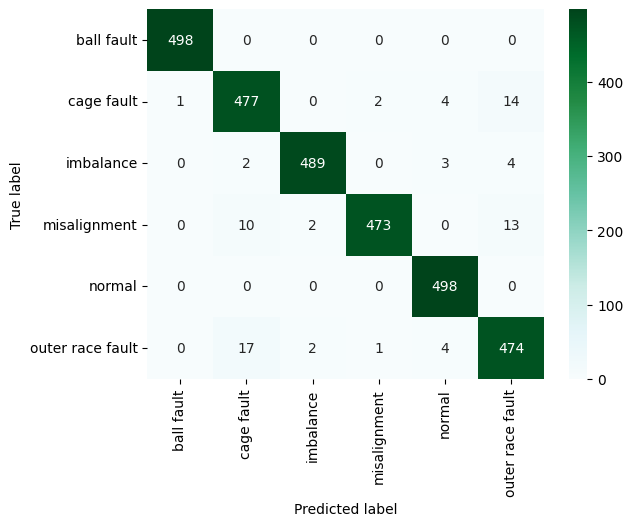
\includegraphics[width=\textwidth]{assets/results/all-features/TD-confusion-matrix.png}
        \caption{Time-domain features}
    \end{subfigure}
    \hfill
    \begin{subfigure}[b]{0.49\textwidth}
        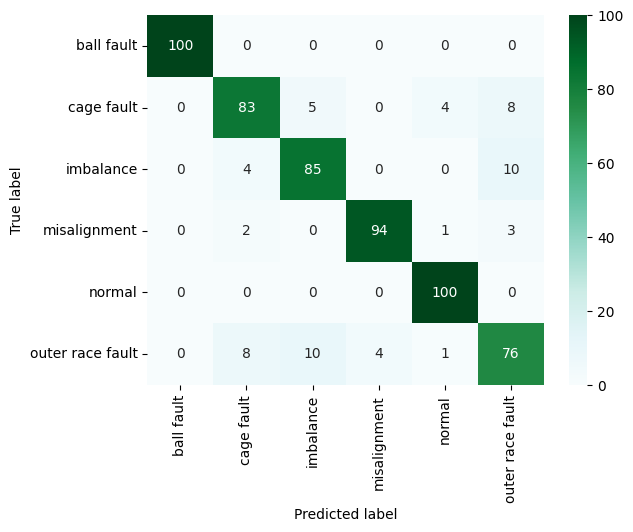
\includegraphics[width=\textwidth]{assets/results/all-features/FD-confusion-matrix.png}
        \caption{Frequency-domain features}
    \end{subfigure}
    \caption{Confusion matrix for complete sets of features}
    \label{fig:evaluation:all-features-confusion-matrix}
\end{figure}

The inner bearing observations are selected to train the k-NN with five neighbours and Euclidean distance metric. The attributes are normalized beforehand, rows are oversampled to a majority label, and data is split into training and testing sets with an 80:20 proportion. The 598 observations of validation data determines the confusion matrix (Fig.~\ref{fig:evaluation:all-features-confusion-matrix}). 

The label ``normal'' is not falsely attributed to other classes in either feature set, but other classes can get assigned to be ``normal''. Most mistakes happen while predicting outer race fault, which gets confused with cage fault, imbalance, and less often with misalignment. The shaft imbalance is applied to simulate bearing faults, which is a natural reason for this high error rate.

\begin{figure}[h]
    \centering
    \begin{subfigure}[b]{0.48\textwidth}
        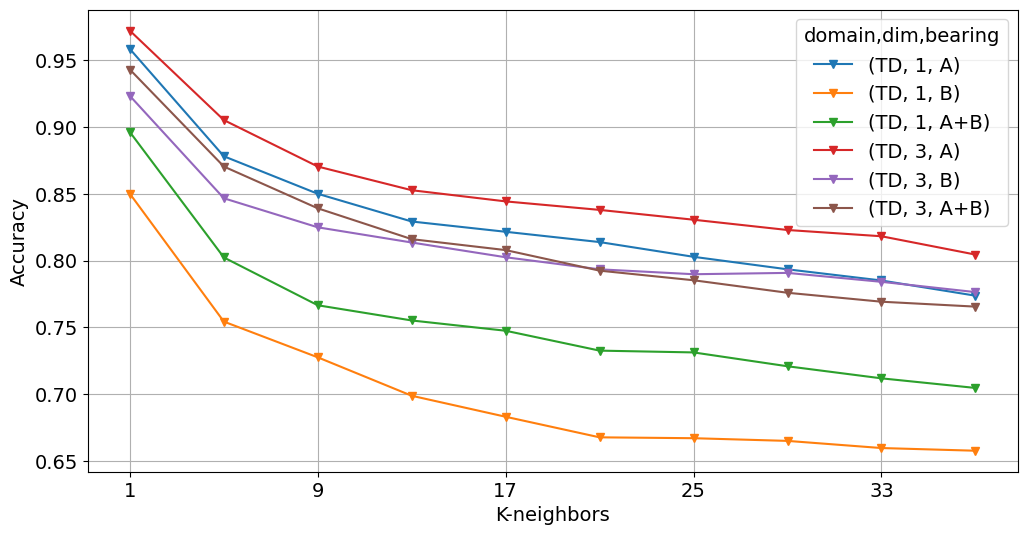
\includegraphics[width=\textwidth]{assets/results/all-features/TD.png}
        \caption{Time-domain features}
    \end{subfigure}
    \hfill
    \begin{subfigure}[b]{0.48\textwidth}
        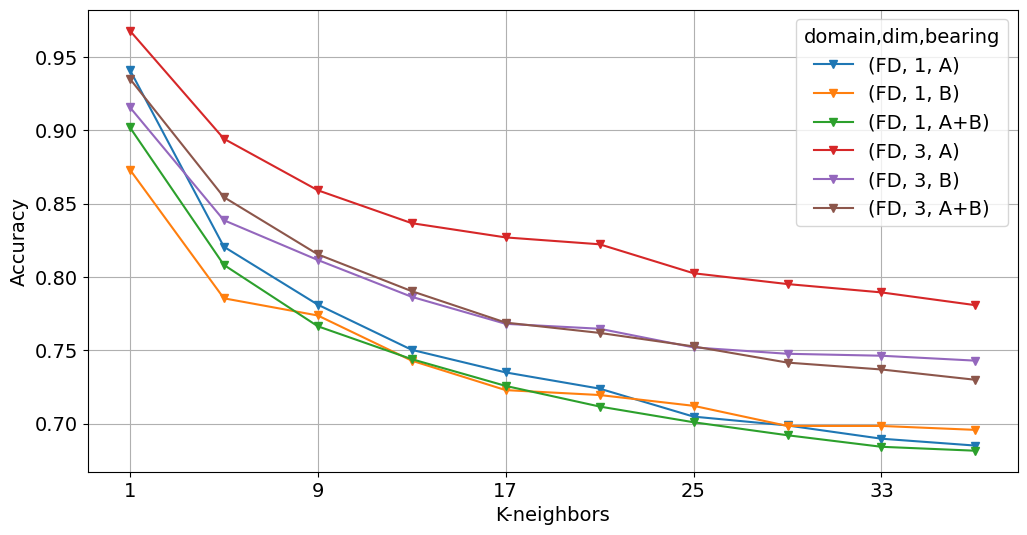
\includegraphics[width=\textwidth]{assets/results/all-features/FD.png}
        \caption{Frequency-domain features}
    \end{subfigure}
    \hfill
    \begin{subfigure}[b]{0.48\textwidth}
        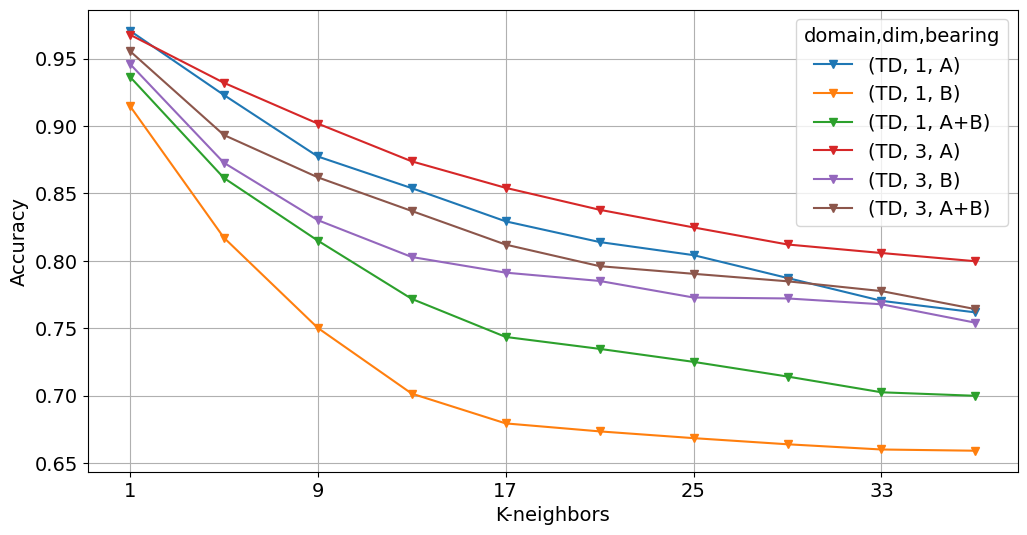
\includegraphics[width=\textwidth]{assets/results/all-features/TD-severity.png}
        \caption{Time-domain features (severity)}
    \end{subfigure}
    \hfill
    \begin{subfigure}[b]{0.48\textwidth}
        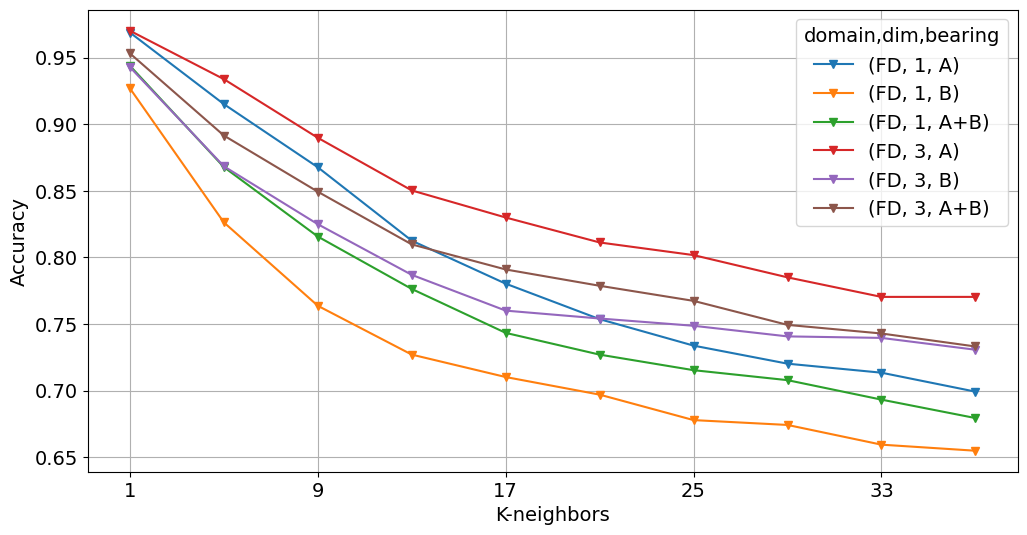
\includegraphics[width=\textwidth]{assets/results/all-features/FD-severity.png}
        \caption{Frequency-domain features (severity)}
    \end{subfigure} 
    \caption{Accuracy on complete feature sets depending on the k-value}
    \label{fig:evaluation:complete-set-k-value}
\end{figure}

An increase in the number of neighbours used for classification in five-fold cross-validated k-NN shows a substantial decrease in accuracy on validation sets (Fig.~\ref{fig:evaluation:complete-set-k-value}). The most prominent drop in performance of around 10\% occurs at the beginning until the k-value of nine, and then the accuracy curve slowly plateaus.

Under every circumstance, the magnitude of the triaxial feature vector reaches better accuracy than those from only the axis of motion for the same source domain and bearing. The model for inner bearing A is more accurate than outer bearing B. The TD set is generally better in predictions than the FD set for the equivalent k-value. The dataset relabeled for high severity has a steeper decrease in accuracy for the same number of neighbours.

\subsection{Feature subset combinations}
The complete sets of predictors are even greatly shrunken to representation that could be presented in 3D plot or in perpendicular cross sections. These trend variables could be used in distinguishing faults the same way as rms amplitude indicates their presence. Each possible combinations of pairs, triplets, and quadruplets construct a separate k-NN model on which prediction accuracy is evaluated. 

\begin{figure}[h]
    \centering
    \begin{subfigure}[b]{0.48\textwidth}
        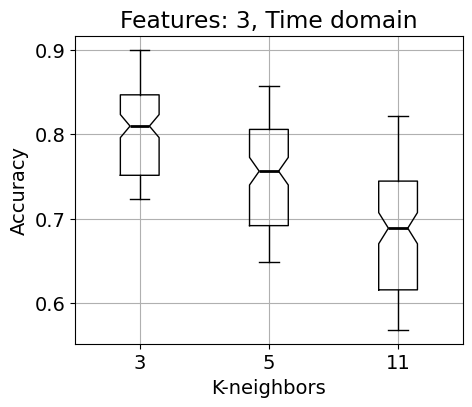
\includegraphics[width=\textwidth]{assets/results/feature-combinations/TD-3-A-False-False-F3.png}
        \caption{Three time-domain features}
    \end{subfigure}
    \hfill
    \begin{subfigure}[b]{0.48\textwidth}
        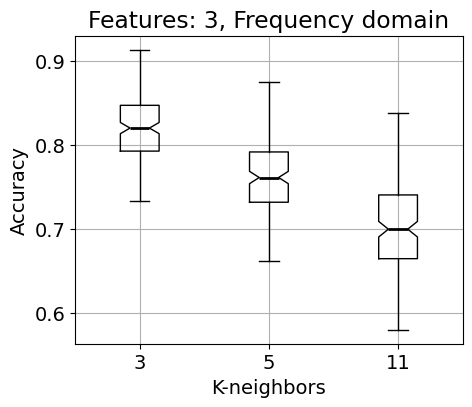
\includegraphics[width=\textwidth]{assets/results/feature-combinations/FD-3-A-False-False-F3.png}
        \caption{Three frequency-domain features}
    \end{subfigure}
    \hfill
    \begin{subfigure}[b]{0.48\textwidth}
        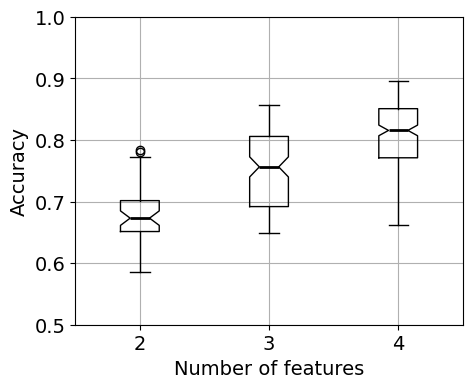
\includegraphics[width=\textwidth]{assets/results/feature-combinations/TD-3-A-False-False-K5.png}
        \caption{Five neighbours in time domain}
    \end{subfigure}
    \hfill
    \begin{subfigure}[b]{0.48\textwidth}
        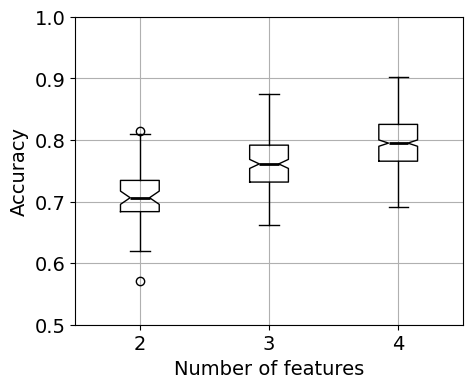
\includegraphics[width=\textwidth]{assets/results/feature-combinations/FD-3-A-False-False-K5.png}
        \caption{Five neighbours in frequency domain}
    \end{subfigure}
    \caption{Model accuracy distribution for bearing A and three axis features}
    \label{fig:evaluation:model-accuracy}
\end{figure}

\begin{figure}[h]
    \centering
    \begin{subfigure}[b]{0.48\textwidth}
        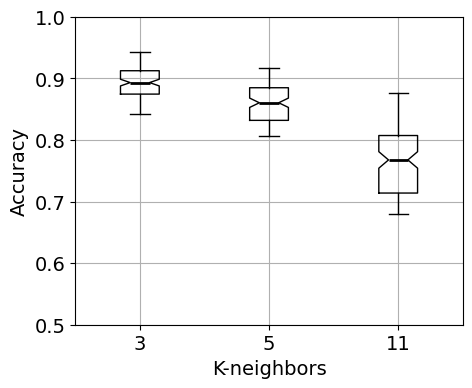
\includegraphics[width=\textwidth]{assets/results/feature-combinations/TD-3-A-True-False-F3.png}
        \caption{Three time-domain features}
    \end{subfigure}
    \hfill
    \begin{subfigure}[b]{0.48\textwidth}
        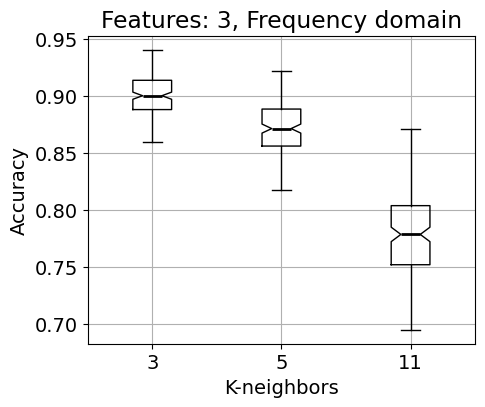
\includegraphics[width=\textwidth]{assets/results/feature-combinations/FD-3-A-True-False-F3.png}
        \caption{Three frequency-domain features}
    \end{subfigure}
    \hfill
    \begin{subfigure}[b]{0.48\textwidth}
        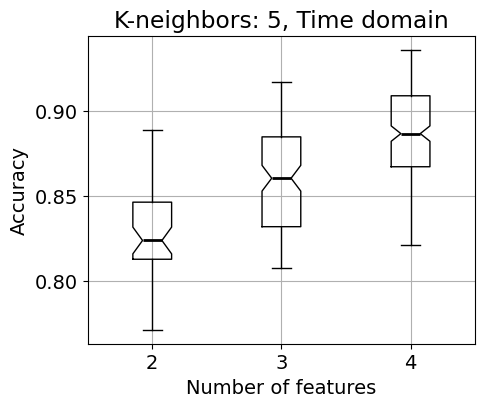
\includegraphics[width=\textwidth]{assets/results/feature-combinations/TD-3-A-True-False-K5.png}
        \caption{Five neighbours in time domain}
    \end{subfigure}
    \hfill
    \begin{subfigure}[b]{0.48\textwidth}
        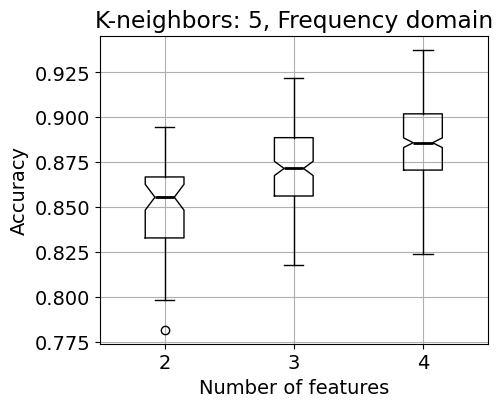
\includegraphics[width=\textwidth]{assets/results/feature-combinations/FD-3-A-True-False-K5.png}
        \caption{Five neighbours in frequency domain}
    \end{subfigure}
    \caption{Model accuracy distribution from bearing A and three axis features after relabeling for high severity faults}
    \label{fig:evaluation:model-accuracy-severity}
\end{figure}

The distribution of model accuracies is documented on features in both domains coined from three dimensions on bearing A with original and high-severity defect labels. The boxplots display the relation of the k-value to accuracy with three features, and the relation of number of features to accuracy with five neighbours (Fig.~\ref{fig:evaluation:model-accuracy-severity} and \ref{fig:evaluation:model-accuracy-severity}).

The decrease in accuracy with additional neighbours is apparent and similar to the trend in complete sets of features. We are interested in comparing maximum accuracies of the accuracy distribution because the optimal feature selection method tries to approach them. The reduction in maximal accuracy is more noticeable between three and five features of 3\% to 5\%, and almost the same amount between five and eleven neighbours. 

The complete sets reach better accuracy than subsets when the number of features is at most three and simultaneously the number of neighbours is five or less. For more triaxial features and more neighbours, the complete set is only about 2\% percent worse at the most than subsets because the curse of dimensionality is not so substantial for ten dimensions.

The spread in model accuracies in the interquartile range is from 5 to 10\%, and measured between whiskers is 25\% at a maximum. The standard deviation is about 7\%. Overall, the time-domain features are better than frequency-domain features for these specific feature spaces.

The number of features has a direct proportionality effect on the optimal model accuracy. An increase from two to three features has more weight than allowing a fourth attribute. The contributions of adding features are around 6\% and 3\%, and the relabeled dataset has an increase of 3\% and 2\%. The absolute accuracies are consecutively for 2, 3, and 4 features when k is equal to 5: 78.31\%, 85.67\%, and 89.55\% for the time domain and 81.52\%, 87.52\%, 90.26\% for the frequency domain.

\subsection{Feature selection techniques}
The predictors chosen with supervised selection strategies are compared to the accuracy distribution of  enumerated combinations of same-sized attribute sets and the performance of its source superset. The metrics for bivariate feature selection are correlation, F statistic, mutual information, and their ensemble by the rank product. The PCA of the complete feature set that retains the same number of features as a selection method is a benchmark to tell whether the linear combination or meaningful attributes get better performance on the MaFaulDa.

\begin{table}[h]
\centering
\begin{adjustbox}{width=\textwidth}
\begin{tabular}{|l|rr|rr|r|l|}
\hline
\multirow{2}{*}{\textbf{Feature set}} & \multicolumn{2}{l|}{\textbf{Accuracy}}                                   & \multicolumn{2}{l|}{\textbf{Percentile}}                 & \multicolumn{1}{l|}{\multirow{2}{*}{\textbf{Domain}}} & \multirow{2}{*}{\textbf{Best features}} \\ \cline{2-5}
                                      & \multicolumn{1}{l|}{\textbf{Train}} & \multicolumn{1}{l|}{\textbf{Test}} & \multicolumn{1}{l|}{\textbf{Train}} & \multicolumn{1}{l|}{\textbf{Test}} & \multicolumn{1}{l|}{}                               &                                         \\ \hline
All features                          & \multicolumn{1}{r|}{96.03}          & 92.80                              & \multicolumn{1}{r|}{100.00}         & 100.00                             & TD                                                   &                                         \\ \hline
PCA PC                                & \multicolumn{1}{r|}{91.20}          & 84.67                              & \multicolumn{1}{r|}{95.00}          & 93.33                              & TD                                                   &                                         \\ \hline
Best features                         & \multicolumn{1}{r|}{91.93}          & 85.47                              & \multicolumn{1}{r|}{100.00}         & 99.17                              & TD                                                   & zerocross, pp, skewness                 \\ \hline
Rank product                          & \multicolumn{1}{r|}{91.21}          & 85.04                              & \multicolumn{1}{r|}{95.83}          & 97.50                              & TD                                                   & zerocross, shape, rms                   \\ \hline
Correlation                           & \multicolumn{1}{r|}{91.21}          & 85.04                              & \multicolumn{1}{r|}{95.83}          & 97.50                              & TD                                                   & shape, zerocross, rms                   \\ \hline
F statistic                           & \multicolumn{1}{r|}{90.59}          & 84.07                              & \multicolumn{1}{r|}{91.67}          & 90.00                              & TD                                                   & rms, pp, zerocross                      \\ \hline
Mutual information                    & \multicolumn{1}{r|}{88.24}          & 80.62                              & \multicolumn{1}{r|}{75.83}          & 76.67                              & TD                                                   & zerocross, shape, crest                 \\ \hline
All features                          & \multicolumn{1}{r|}{93.67}          & 88.45                              & \multicolumn{1}{r|}{100.00}         & 100.00                             & FD                                                  &                                         \\ \hline
PCA PC                                & \multicolumn{1}{r|}{86.76}          & 78.51                              & \multicolumn{1}{r|}{64.85}          & 70.91                              & FD                                                   &                                         \\ \hline
Best features                         & \multicolumn{1}{r|}{92.86}          & 87.52                              & \multicolumn{1}{r|}{100.00}         & 100.00                             & FD                                                   & centroid, roll\_off, entropy            \\ \hline
Rank product                          & \multicolumn{1}{r|}{85.79}          & 77.18                              & \multicolumn{1}{r|}{51.52}          & 57.58                              & FD                                                   & roll\_off, flux, skewness               \\ \hline
Correlation                           & \multicolumn{1}{r|}{85.79}          & 77.18                              & \multicolumn{1}{r|}{51.52}          & 57.58                              & FD                                                   & roll\_off, skewness, flux               \\ \hline
F statistic                           & \multicolumn{1}{r|}{85.79}          & 77.18                              & \multicolumn{1}{r|}{51.52}          & 57.58                              & FD                                                   & roll\_off, flux, skewness               \\ \hline
Mutual information                    & \multicolumn{1}{r|}{90.73}          & 83.60                              & \multicolumn{1}{r|}{94.55}          & 94.55                              & FD                                                   & roll\_off, entropy, noisiness           \\ \hline
\end{tabular}
\end{adjustbox}
\caption{Feature selection method accuracy and percentile within accuracy distribution of all three member subsets. (bearing = A, dimension = 3, k=5)}
\label{tab:evaluation:fsel}
\end{table}

\begin{table}[h]
\centering
\begin{adjustbox}{width=\textwidth}
\begin{tabular}{|l|rr|rr|r|l|}
\hline
\multirow{2}{*}{\textbf{Feature set}} & \multicolumn{2}{l|}{\textbf{Accuracy}}                                   & \multicolumn{2}{l|}{\textbf{Percentile}}                 & \multicolumn{1}{l|}{\multirow{2}{*}{\textbf{Domain}}} & \multirow{2}{*}{\textbf{Best features}} \\ \cline{2-5}
                                      & \multicolumn{1}{l|}{\textbf{Train}} & \multicolumn{1}{l|}{\textbf{Test}} & \multicolumn{1}{l|}{\textbf{Train}} & \multicolumn{1}{l|}{\textbf{Test}} & \multicolumn{1}{l|}{}                               &                                         \\ \hline
All features                          & \multicolumn{1}{r|}{96.42}          & 94.76                              & \multicolumn{1}{r|}{100.00}         & 100.00                             & TD                                                   &                                         \\ \hline
PCA PC                                & \multicolumn{1}{r|}{94.63}          & 92.07                              & \multicolumn{1}{r|}{100.00}         & 100.00                             & TD                                                   &                                         \\ \hline
Best features                         & \multicolumn{1}{r|}{94.58}          & 91.71                              & \multicolumn{1}{r|}{100.00}         & 99.17                              & TD                                                   & zerocross, aac, shape                   \\ \hline
Rank product                          & \multicolumn{1}{r|}{94.31}          & 91.40                              & \multicolumn{1}{r|}{98.33}          & 95.83                              & TD                                                   & zerocross, shape, rms                   \\ \hline
Correlation                           & \multicolumn{1}{r|}{94.31}          & 91.40                              & \multicolumn{1}{r|}{98.33}          & 95.83                              & TD                                                   & zerocross, shape, rms                   \\ \hline
F statistic                           & \multicolumn{1}{r|}{94.31}          & 91.40                              & \multicolumn{1}{r|}{98.33}          & 95.83                              & TD                                                   & shape, zerocross, rms                   \\ \hline
Mutual information                    & \multicolumn{1}{r|}{91.90}          & 88.51                              & \multicolumn{1}{r|}{72.50}          & 76.67                              & TD                                                   & zerocross, shape, clearance             \\ \hline
All features                          & \multicolumn{1}{r|}{95.20}          & 93.20                              & \multicolumn{1}{r|}{100.00}         & 100.00                             & FD                                                   &                                         \\ \hline
PCA PC                                & \multicolumn{1}{r|}{92.14}          & 88.84                              & \multicolumn{1}{r|}{69.09}          & 73.94                              & FD                                                   &                                         \\ \hline
Best features                         & \multicolumn{1}{r|}{94.64}          & 91.94                              & \multicolumn{1}{r|}{100.00}         & 99.39                              & FD                                                   & centroid, roll\_off, entropy            \\ \hline
Rank product                          & \multicolumn{1}{r|}{93.89}          & 91.24                              & \multicolumn{1}{r|}{95.15}          & 97.58                              & FD                                                   & entropy, noisiness, centroid            \\ \hline
Correlation                           & \multicolumn{1}{r|}{94.50}          & 92.19                              & \multicolumn{1}{r|}{99.39}          & 100.00                             & FD                                                   & entropy, centroid, flux                 \\ \hline
F statistic                           & \multicolumn{1}{r|}{94.50}          & 92.19                              & \multicolumn{1}{r|}{99.39}          & 100.00                             & FD                                                   & entropy, flux, centroid                 \\ \hline
Mutual information                    & \multicolumn{1}{r|}{93.32}          & 90.67                              & \multicolumn{1}{r|}{90.91}          & 91.52                              & FD                                                   & noisiness, roll\_off, entropy           \\ \hline
\end{tabular}
\end{adjustbox}
\caption{Feature selection method accuracy and percentile within accuracy distribution of all three member subsets. (severity, bearing = A, dimension = 3, k=5)}
\label{tab:evaluation:fsel-severity}
\end{table}

Table~\ref{tab:evaluation:fsel} compares the concrete case of choosing the three features from each domain on bearing A and k-NN with five neighbours. Table~\ref{tab:evaluation:fsel-severity} uses labels for high-severity faults. There is a significant difference in train and test accuracy, which means the model is likely overfitting. The percentile within the distribution is measured to its respective data, the train or validation set. However, the percentile of best features in the test data is calculated against distribution of the training data.

Combining the rankings from several metrics is necessary to get consistent results. This is evidenced by the variability in the success of selected feature sets in final prediction performance under multiple conditions. The PCA with three components for the complete feature sets is comparable in accuracy to selection methods with original attributes.

The triplet of variables with the best results is in TD set: zero-crossing rate, peak-to-peak, skewness, and in FD set: centroid, roll-off, and entropy. With high severity labels, the best attributes for FD stay the same, but average amplitude change and shape factor are preferred along the zero-crossing rate. The rank product picked up roll-off, flux, and skewness for the FD set, which is suboptimal. The two of the three methods in the ensemble arrive at the same set overruling the superior set produced by mutual information. In the TD set, the zero-crossing rate, shape, and rms, are chosen by rank product. 

\begin{figure}[h]
    \centering
    \begin{subfigure}[b]{0.48\textwidth}
        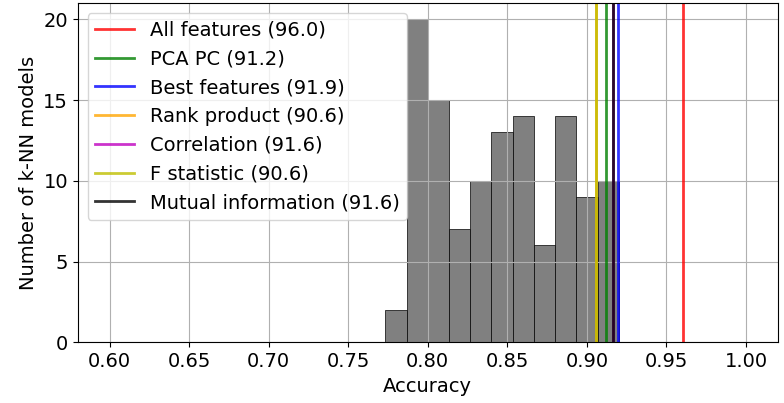
\includegraphics[width=\textwidth]{assets/results/feature-combinations/model-distr-fsel-k5-f3-TD-train.png}
        \caption{Time-domain features (train)}
    \end{subfigure}
    \hfill
    \begin{subfigure}[b]{0.48\textwidth}
        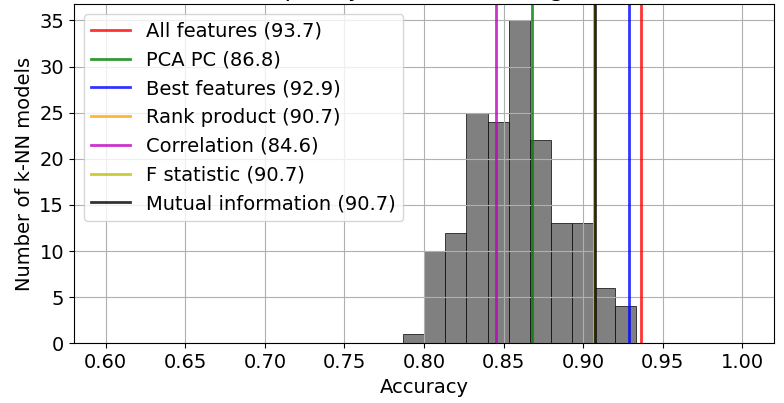
\includegraphics[width=\textwidth]{assets/results/feature-combinations/model-distr-fsel-k5-f3-FD-train.png}
        \caption{Frequency-domain features (train)}
    \end{subfigure}
    \hfill
    \begin{subfigure}[b]{0.48\textwidth}
        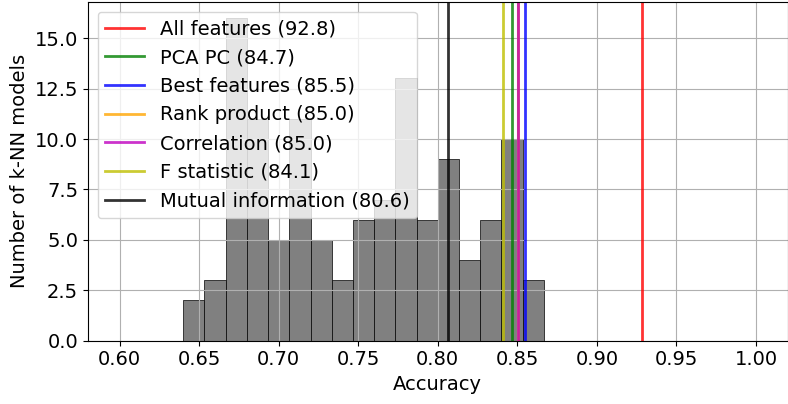
\includegraphics[width=\textwidth]{assets/results/feature-combinations/model-distr-fsel-k5-f3-TD-test.png}
        \caption{Time-domain features (test)}
    \end{subfigure}
    \hfill
    \begin{subfigure}[b]{0.48\textwidth}
        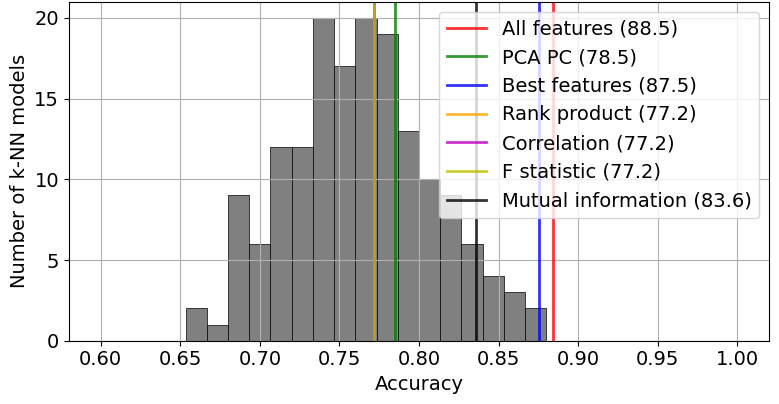
\includegraphics[width=\textwidth]{assets/results/feature-combinations/model-distr-fsel-k5-f3-FD-test.png}
        \caption{Frequency-domain features (test)}
    \end{subfigure}
    \caption{Model accuracy statistical distributions with feature selection methods for three predictors (k = 5)}
    \label{fig:evaluation:fsel-model-distr}
\end{figure}

The entire accuracy distribution for the training and testing set with original labels is drawn as a histogram (Fig.~\ref{fig:evaluation:fsel-model-distr}). The results of the chosen predictors are mapped out onto the distribution as vertical lines that stack up near the maximum for the time domain or disperse slightly above the median for the frequency domain. The accuracy of all features is unreachable for three feature subsets. Another noticeable difference between distributions is their shift down and greater spread in testing sets compared to training sets.

\begin{table}[]
\centering
\begin{adjustbox}{width=\textwidth}
\begin{tabular}{|l|r|r|}
\hline
\textbf{Method}    & \multicolumn{1}{l|}{\textbf{Median percentile {[}\%{]}}} & \multicolumn{1}{l|}{\textbf{Median accuracy {[}\%{]}}} \\ \hline
Rank product       & 88.97                                                    & 79.82                                                 \\ \hline
Mutual information & 91.81                                                    & 80.87                                                 \\ \hline
F statistic        & 86.90                                                    & 79.63                                                 \\ \hline
Correlation        & 84.49                                                    & 79.04                                                  \\ \hline
\end{tabular}
\end{adjustbox}
\caption{Feature selection methods evaluated in summary over all experimental conditions}
\label{tab:evaluation:compare-fsel-accuracy}
\end{table}

\begin{table}[]
\centering
\begin{adjustbox}{width=\textwidth}
\begin{tabular}{|l|r|r|r|}
\hline
                            & \multicolumn{1}{l|}{\textbf{Best in scenarios}} & \multicolumn{1}{l|}{\textbf{Scenarios {[}\%{]}}} & \multicolumn{1}{l|}{\textbf{Mean percentile {[}\%{]}}} \\ \hline
\textbf{Rank product}       & 94                                                     & 43.52                                            & 92.38 \\ \hline
\textbf{Mutual information} & 87                                                      & 40.28                                            & 91.79 \\ \hline
\textbf{Correlation}        & 26                                                      & 12.04                                             & 97.54 \\ \hline
\textbf{F statistic}        & 9                                                       & 4.16                                             & 96.10 \\ \hline
\textbf{$\Sigma$}           & 216                                                     & 100                                       & -                                                      \\ \hline
\end{tabular}
\end{adjustbox}
\caption{The experimental scenarios in which the method is found to be the best}
\label{tab:evaluation:best-selection-method}
\end{table}

\begin{figure}[t]
    \centering
    \begin{subfigure}[b]{0.48\textwidth}
        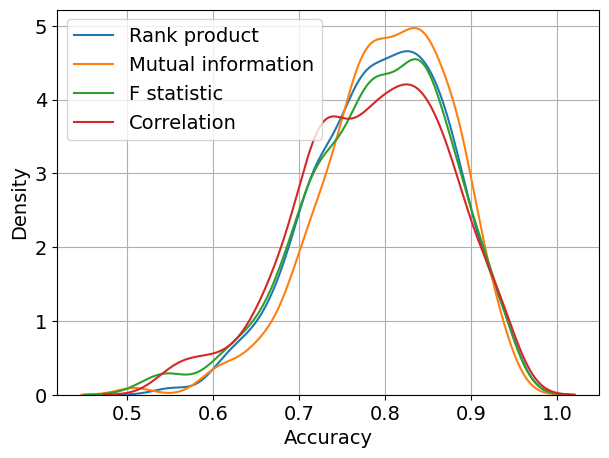
\includegraphics[width=\textwidth]{assets/results/feature-combinations/fsel-accuracy.png}
        \caption{Accuracy}
    \end{subfigure}
    \hfill
    \begin{subfigure}[b]{0.48\textwidth}
        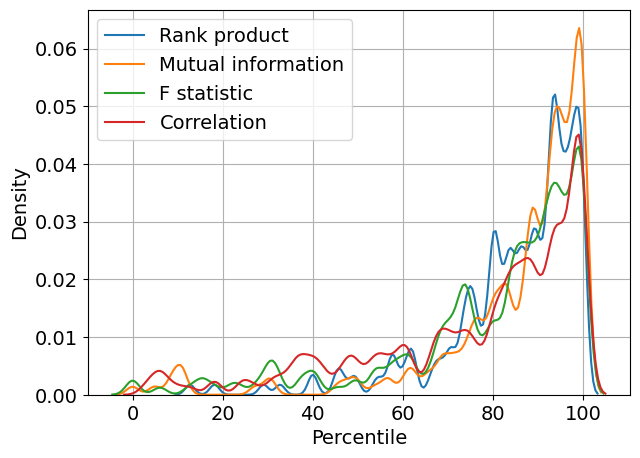
\includegraphics[width=\textwidth]{assets/results/feature-combinations/fsel-percentile.png}
        \caption{Percentile in distribution of accuracies}
    \end{subfigure}
    \caption{Quality of choice for feature selection methods}
    \label{fig:evaluation:kde-fsel-perecentile}
\end{figure}

\begin{figure}[t]
    \centering
    \begin{subfigure}[b]{0.24\textwidth}
        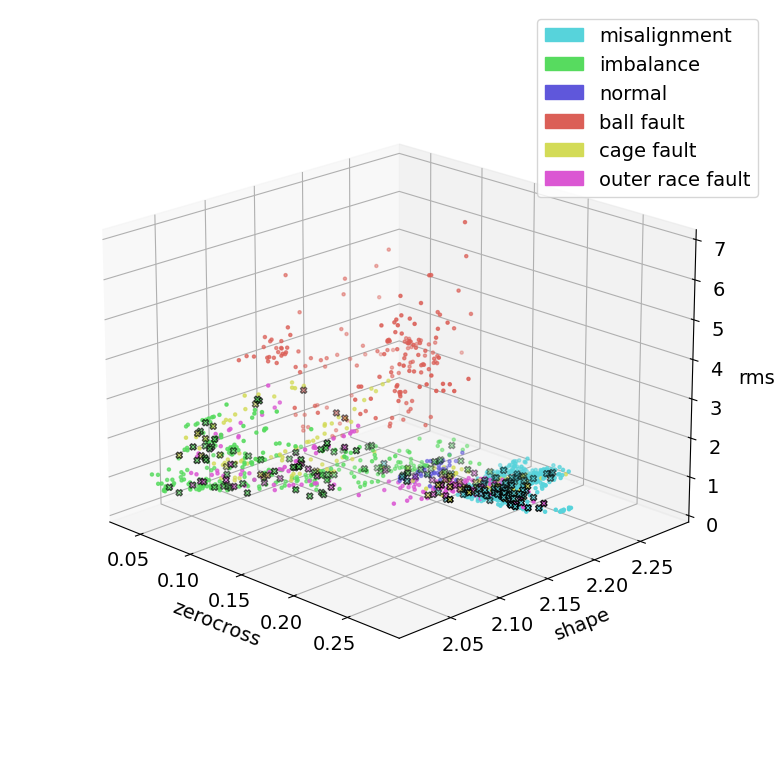
\includegraphics[width=\textwidth]{assets/results/labels/TD.png}
        \caption{TD [89.05\%]}
    \end{subfigure}
    \hfill
    \begin{subfigure}[b]{0.24\textwidth}
        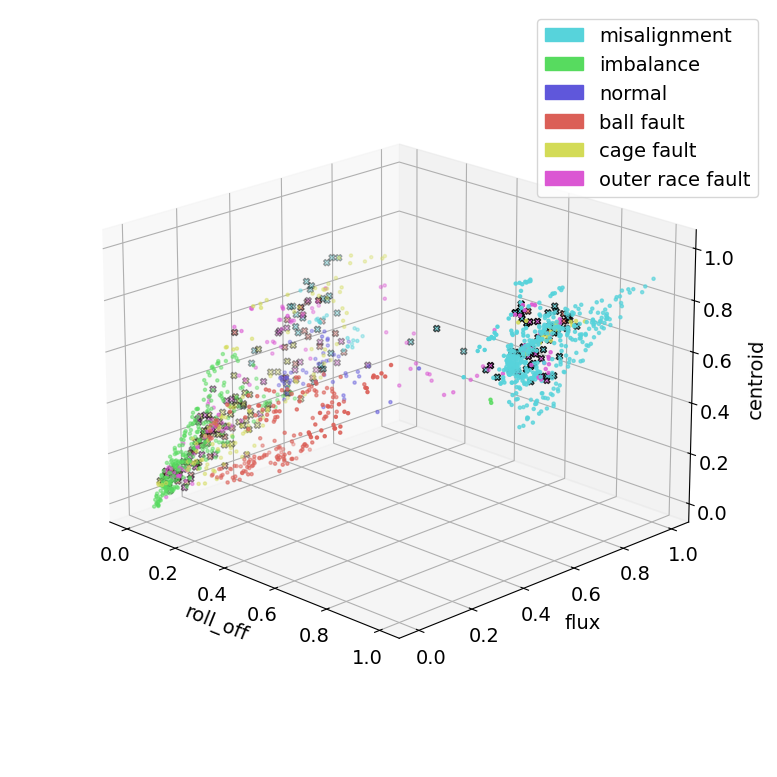
\includegraphics[width=\textwidth]{assets/results/labels/FD.png}
        \caption{FD [77.18\%]}
    \end{subfigure}
    \hfill
    \begin{subfigure}[b]{0.24\textwidth}
        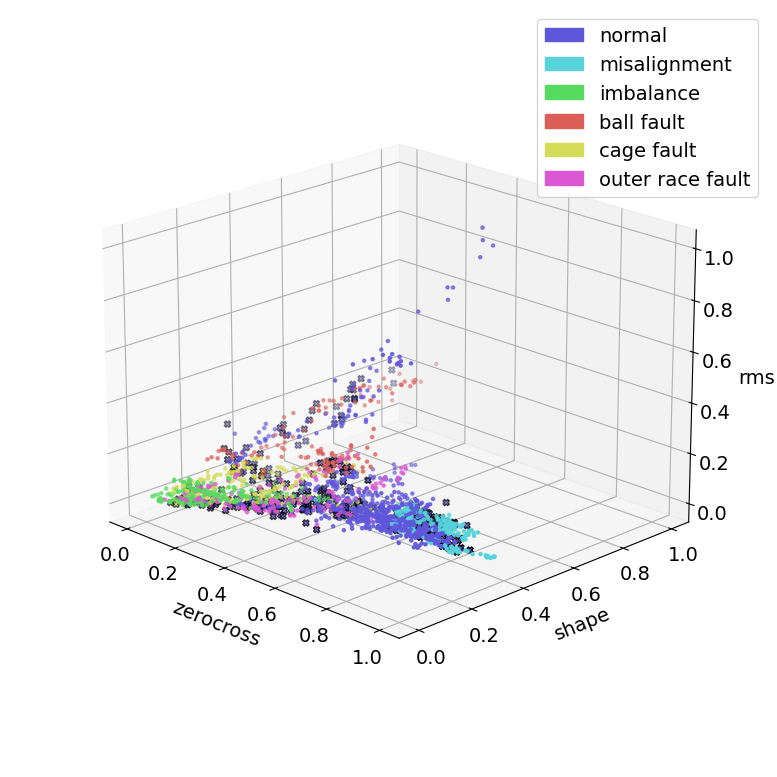
\includegraphics[width=\textwidth]{assets/results/labels/TD-severity.png}
        \caption{TD (s) [91.40\%]}
    \end{subfigure}
    \hfill
    \begin{subfigure}[b]{0.24\textwidth}
        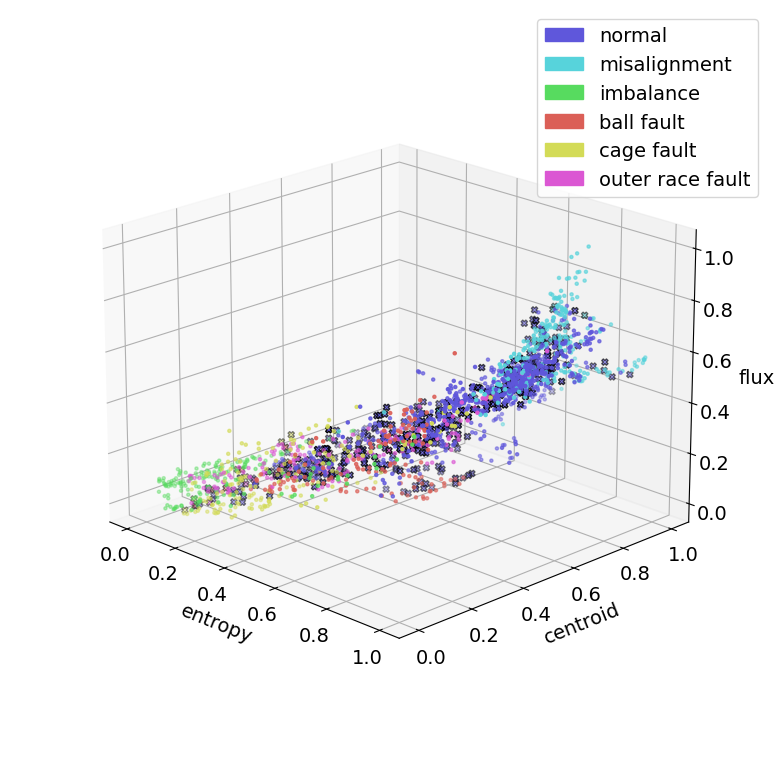
\includegraphics[width=\textwidth]{assets/results/labels/FD-severity.png}
        \caption{FD (s) [91.24\%]}
    \end{subfigure} 
    \caption{Three features in both domains chosen by rank product with prediction accuracy in brackets. Relabeled dataset is marked with (s)}
\end{figure}


In 216 scenarios, the mutual information has better median accuracy (80.87\%) and distribution percentile (91.81\%) followed by rank product with an accuracy of 79.82\% of and percentile of 88.97\% (Tab.~\ref{tab:evaluation:compare-fsel-accuracy}). The scenarios are composed of 24 base dataset modifications and options for hyperparameters k-value and number of features. 

The rank product is the best method in the majority of 43.52\% scenarios. Mutual information comes second in 40.28\% cases, where it is deemed the best strategy (Tab.~\ref{tab:evaluation:best-selection-method}). The median accuracy, in cases where they are the best method, is also better for rank product 92.38\% compared to 91.79\% mutual information. 

Kernel density estimate plot (Fig.~\ref{fig:evaluation:kde-fsel-perecentile}) shows the distribution of accuracies for the selection methods and percentiles for predictor subsets they choose. The feature selection usually picks variables so that they stay in the upper quartile of the distribution above the 75\% percentile. The median accuracy of all methods is the vicinity of 80\%.

The features chosen by rank product are visualized as a three-dimensional scatter plot. The colors of data points represent correct labels with ex marks for misses. The scales on graph axes are inverse transformed of the min-max scaler. The visualization of predicted groups suggests another transform should be applied to even out the distances and handle the outliers.


\subsection{Incremental learning}
Online learning imitates hardened conditions for machinery diagnostics that appear in deployment. Delayed provision or omission of actual labels undoubtedly degrades the reliability of the classification. The question is how quickly the accuracy approaches the optimal one from the nearest neighbors trained in batch and what is the effect on the classifier from routine difficulties associated with the continuous labeling process.

\begin{figure}[ht]
    \centering
    \begin{subfigure}[b]{0.32\textwidth}
        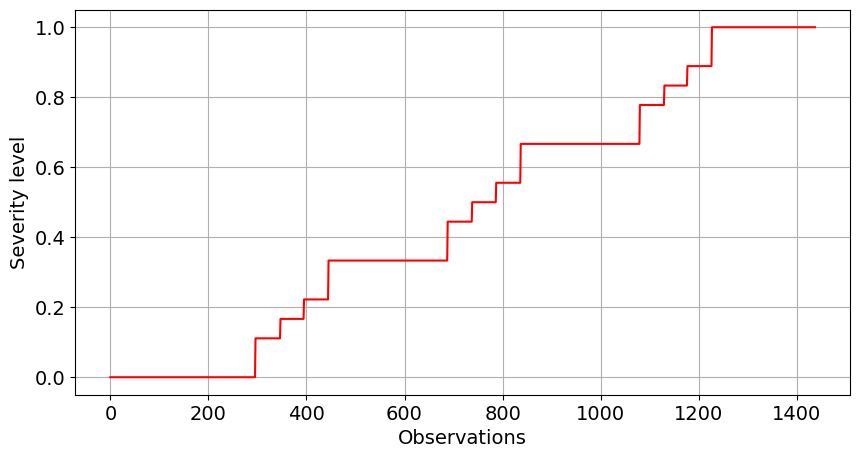
\includegraphics[width=\textwidth]{assets/results/incremental-learning/severity-levels.png}
        \caption{Relative severity levels}
        \label{fig:design:online-count-severity-level}
    \end{subfigure}
    \hfill
    \begin{subfigure}[b]{0.32\textwidth}
        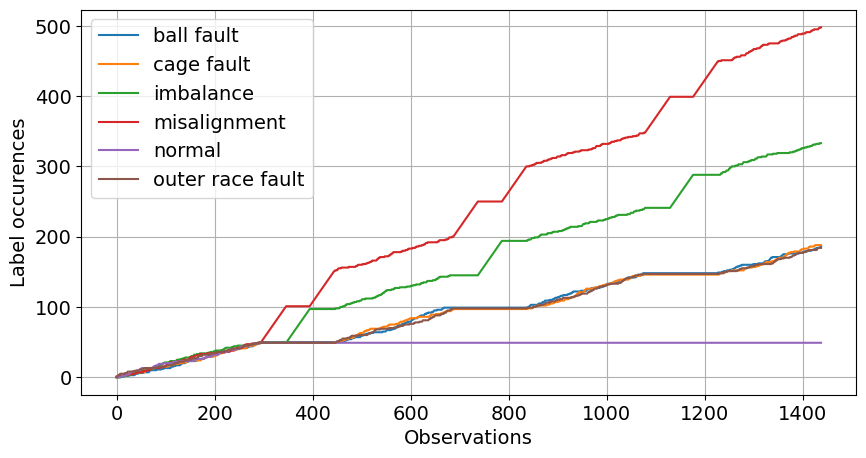
\includegraphics[width=\textwidth]{assets/results/incremental-learning/order-natural.png}
        \caption{Original labels}
        \label{fig:design:online-event-order}
    \end{subfigure}
    \hfill
    \begin{subfigure}[b]{0.32\textwidth}
        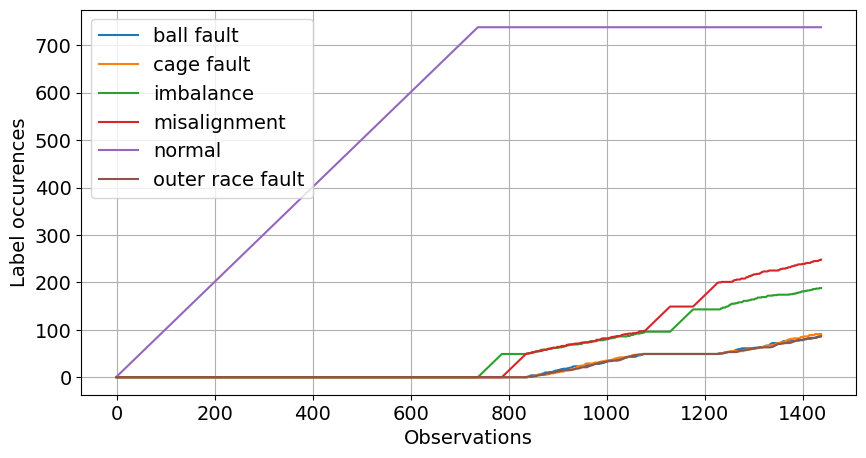
\includegraphics[width=\textwidth]{assets/results/incremental-learning/order-severity.png}
        \caption{High severity labels}
         \label{fig:design:online-event-order-severity}
    \end{subfigure}
    \caption{Ordering of faults in dataset according to relative severity levels}
\end{figure}

The k-NN models in incremental learning experiments train on the same base training dataset as those in batch learning for bearing A. Online learning metrics are evaluated by progressive valuation on a still unbalanced dataset. In this manner, we can compare the training accuracies for the last sample of online models to their batch counterparts.

The \textbf{stream of events} is ordered by rising severity levels (Fig.~\ref{fig:design:online-count-severity-level}), which ensures steady increments in label counts throughout the simulation (Fig.~\ref{fig:design:online-event-order}). The same sorting approach is applied to the dataset where low-severity faults are annotated as baseline. During most of its lifespan, the machine simulator looks to be in a fine operating state. Near the end of the simulation, faults start to develop (Fig.~\ref{fig:design:online-event-order-severity}). These artificially streamed event sequences are a bit unrealistic because all types of faults never begin to appear simultaneously with equal strengths. It is meant to approximate the gradual overall degradation of the machine.

A significant change in the data stream occurs after 294 out of 1438 observations (or after 737 for high severity faults) when all 49 (or 737) normal conditions are consumed in the training process. Counters of other faults show that predictions are skewed towards more represented classes of imbalance and misalignment. The uneven evolution of categories in a stream impacts the evolution of accuracy in the remaining experiments. The test accuracies of comparable batch models for three best features are 85.47\% (TD), 87.52\% (FD), 91.71\% (TD severity), and 91.94\% (FD severity).

\begin{figure}[]
    \centering
    \begin{subfigure}[b]{0.48\textwidth}
        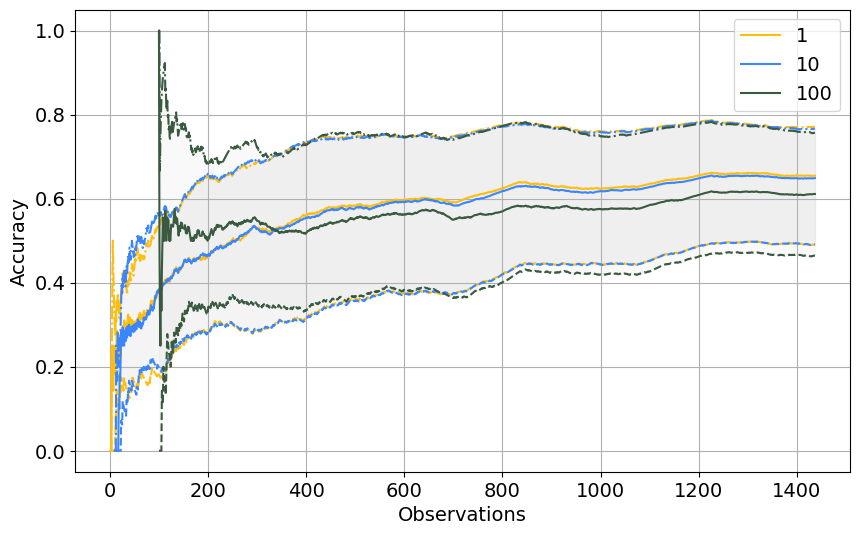
\includegraphics[width=\textwidth]{assets/results/incremental-learning/tumbling-TD.png}
        \caption{Time-domain features}
    \end{subfigure}
    \hfill
    \begin{subfigure}[b]{0.48\textwidth}
        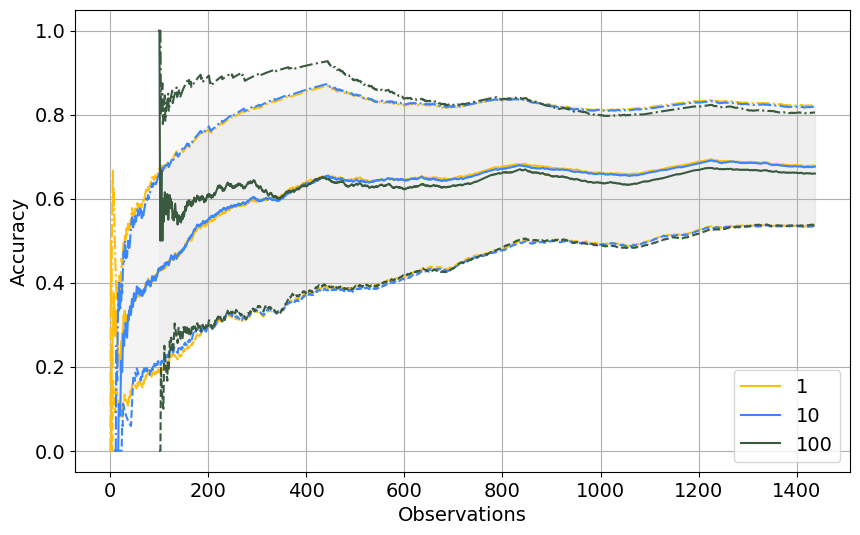
\includegraphics[width=\textwidth]{assets/results/incremental-learning/tumbling-FD.png}
        \caption{Frequency-domain features}
    \end{subfigure}
    \hfill
    \begin{subfigure}[b]{0.48\textwidth}
        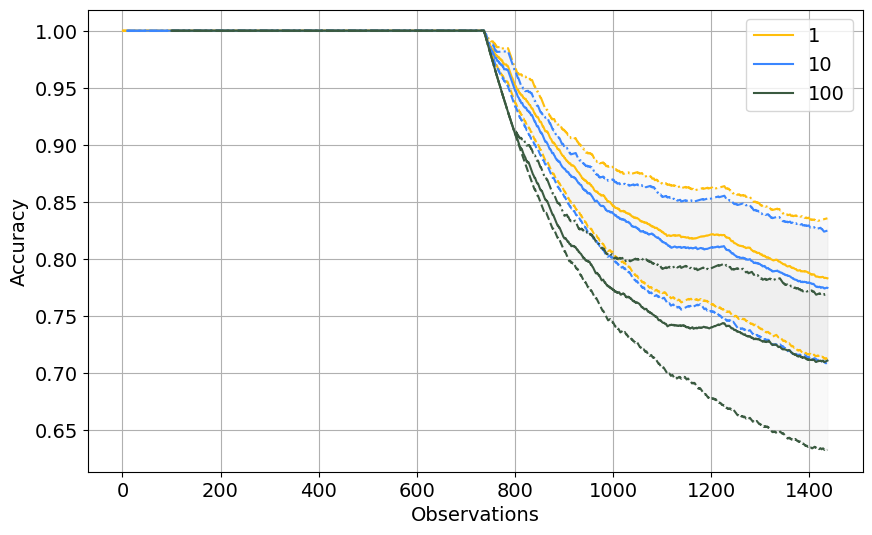
\includegraphics[width=\textwidth]{assets/results/incremental-learning/tumbling-TD-severity.png}
        \caption{Time-domain features (severity)}
    \end{subfigure}
    \hfill
    \begin{subfigure}[b]{0.48\textwidth}
        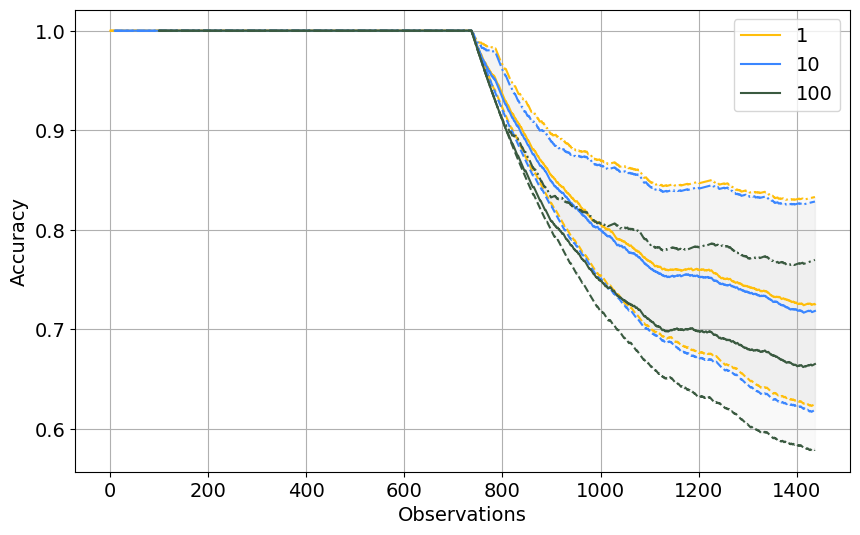
\includegraphics[width=\textwidth]{assets/results/incremental-learning/tumbling-FD-severity.png}
        \caption{Frequency-domain features (severity)}
    \end{subfigure} 
    \caption{Tumbling window of lengths 1, 10, 100 during incremental learning}
    \label{fig:evaluation:tumbling-window-online}
\end{figure}

\begin{figure}[]
    \centering
    \begin{subfigure}[b]{0.48\textwidth}
        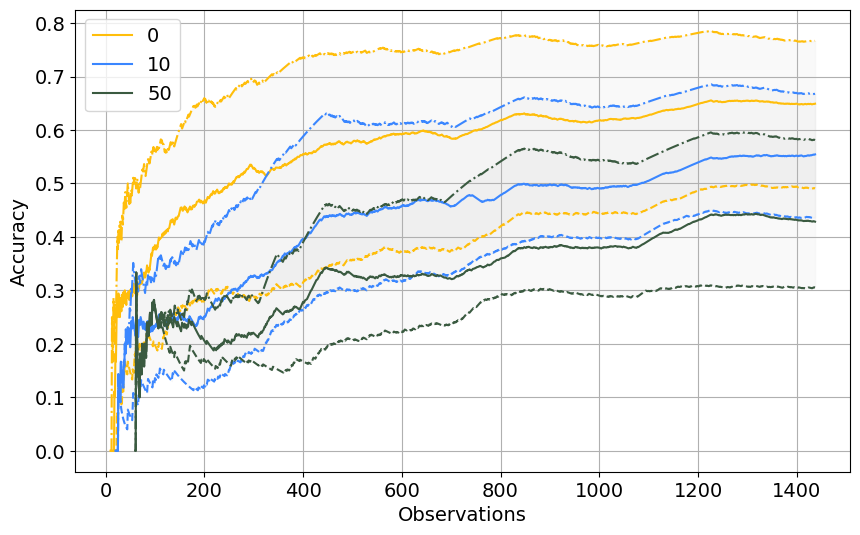
\includegraphics[width=\textwidth]{assets/results/incremental-learning/skip-label-TD.png}
        \caption{Time-domain features}
    \end{subfigure}
    \hfill
    \begin{subfigure}[b]{0.48\textwidth}
        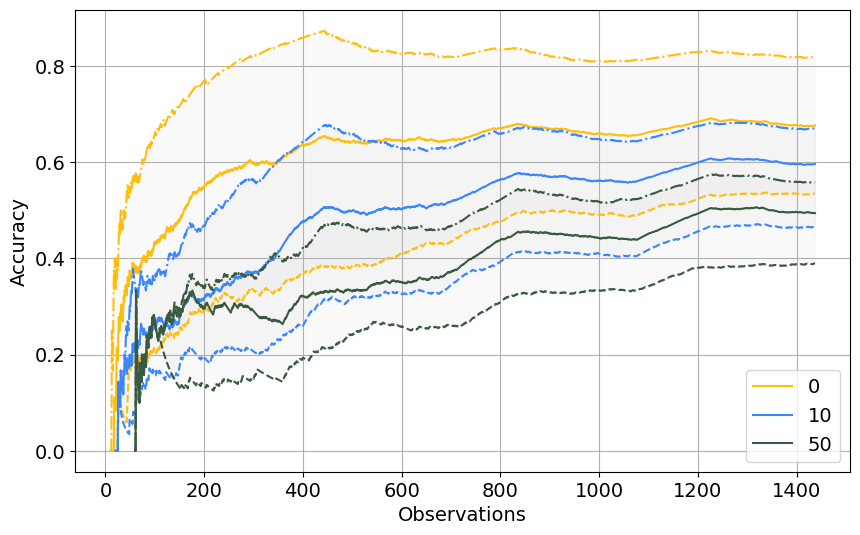
\includegraphics[width=\textwidth]{assets/results/incremental-learning/skip-label-FD.png}
        \caption{Frequency-domain features}
    \end{subfigure}
    \hfill
    \begin{subfigure}[b]{0.48\textwidth}
        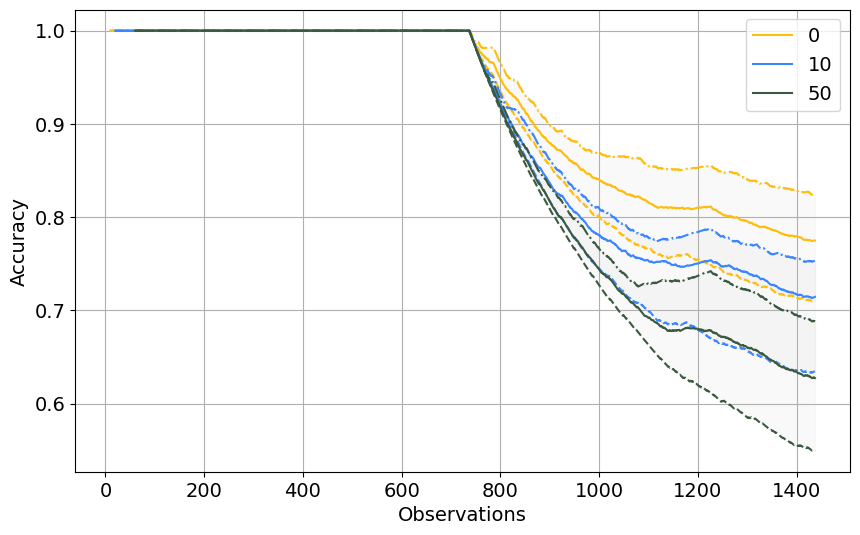
\includegraphics[width=\textwidth]{assets/results/incremental-learning/skip-label-TD-severity.png}
        \caption{Time-domain features (severity)}
    \end{subfigure}
    \hfill
    \begin{subfigure}[b]{0.48\textwidth}
        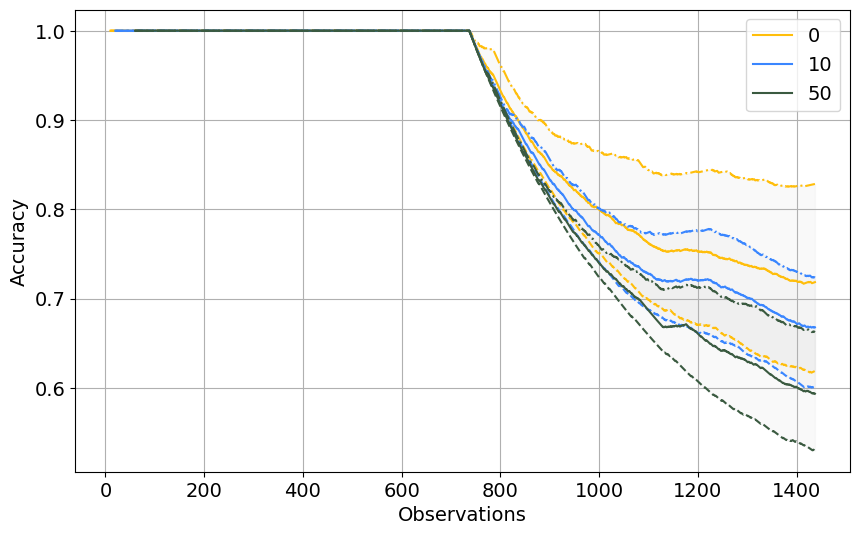
\includegraphics[width=\textwidth]{assets/results/incremental-learning/skip-label-FD-severity.png}
        \caption{Frequency-domain features (severity)}
    \end{subfigure} 
    \caption{Omission of labels during incremental learning with tumbling window of length 10 and gaps of size 0, 10, and 50 samples}
    \label{fig:evaluation:label-skips-online}
\end{figure}

During gradual learning, the correct labels are supplied in bulk at a fixed period. Labeling delay in \textbf{tumbling window} decreases towards the window's end. Figure~\ref{fig:evaluation:tumbling-window-online} plots the evolution of the k-NN model's distribution of accuracy for windows of size 1, 10, and 100 observations. The models consist of three predictors and use five neighbours for prediction. Each window length is described with three curves of identical colour. The median is drawn with a solid line, the maximum with a dash-dotted line, and the minimum with a dashed line.

Initial zero accuracy is caused by a warming-up period in data collection during the span of the first few windows. The true labels are unknown at that point. After just a handful of windows in the beginning, accuracy jumps above 60\% for the best triplet of attributes and stabilizes after 400 observations. In an alternative labeling scheme, the accuracy for one class is 100\% and only after encountering other fault types, it decreases to a level above 75\% for the best set.

The top accuracies after sequentially seeing samples in the longest tumbling windows of 100 observations are 75.71\% (TD), 76.98\% (FD), 76.98\% (TD severity), and 80.56\% (FD severity). The degradations in accuracy when compared to the batch model are by 9.76\% (TD), 10.54\% (FD), 14.73\% (TD severity), and 11.38\% (FD severity). The effect of severe performance hit could be attributed to unbalanced data based on the analysis chapter. The online multiclass oversampling method would need to be inserted into the pipeline to prove this hypothesis.

Labeling every \nth{10} sample (10\% of the dataset) with a tumbling window of 10 samples reduces maximum accuracy for the three-predictor model compared to data points without gaps in labels. In time-domain features, it is decreased by 9.9\% to 66.78\%, and by 14.93\% in frequency-domain features to 67.00\% (Fig.~\ref{fig:evaluation:label-skips-online}). More annotations can be scrapped in the case of a relabeled dataset where keeping just 0.02\% of the class labels produces a decrease by 13.7\% to 68.79\% for time domain attributes, and by 16.59\% to 66.25\% for frequency domain attributes.


\section{Industrial dataset analysis}
The latter part of the solution evaluation focuses on signal properties of vibrations from air compressors, water pumps, and electric induction motors. Our custom dataset is compiled from measurements collected during regular operation of machines. The behaviour of different machines is compared using static frequency estimations and time-frequency spectrograms. The domain expert methodology is carried out to diagnose the current status of water pumps. The presence of fault is confronted with sensor logs from the pump's vendor.

\subsection{Data logger verification}
Data logger capabilities were verified by capturing vibrations on the back of the plastic casing for the electric motor of the standing fan. The recorder is able to run continuously for more than one minute without dropping any samples. The amplitude range after conversion is constrained in the expected range (Fig.~\ref{fig:evaluation:logger-waveform}). The same amplitudes were obtained previously on a proof-of-concept device using analog accelerometer ADXL335 on BeagleBone Black, albeit with lower sensitivity.

\begin{figure}[h]
    \centering
    \begin{subfigure}[b]{0.49\textwidth}
        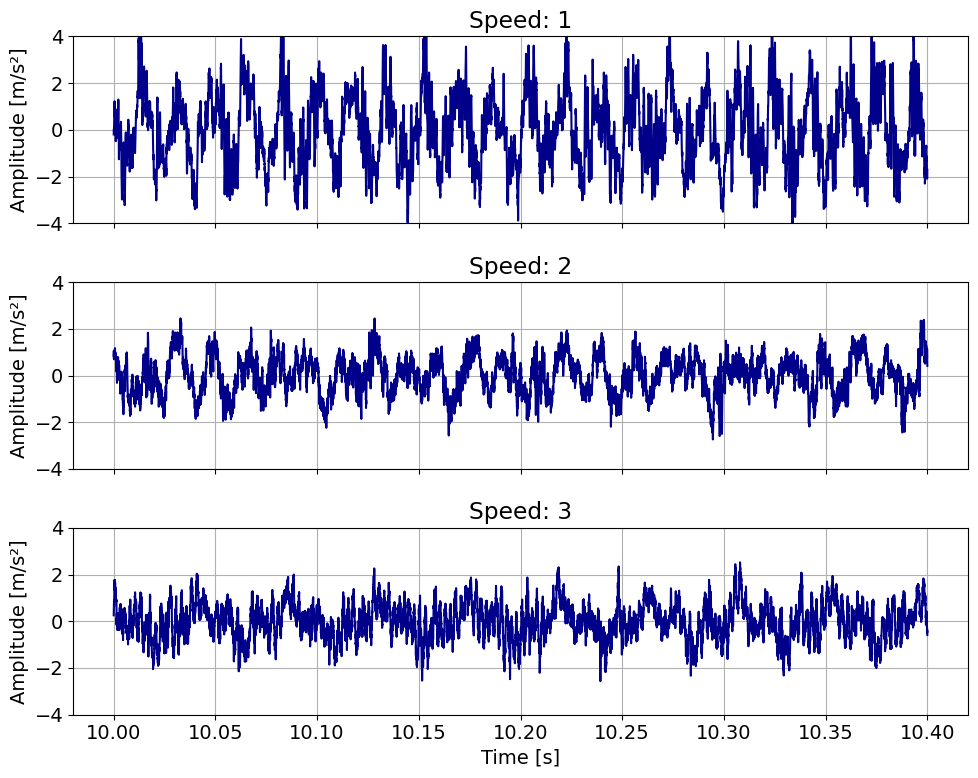
\includegraphics[width=\textwidth]{assets/results/standing-fan/waveform.png}
        \caption{Time waveform}
        \label{fig:evaluation:logger-waveform}
    \end{subfigure}
    \hfill
    \begin{subfigure}[b]{0.49\textwidth}
        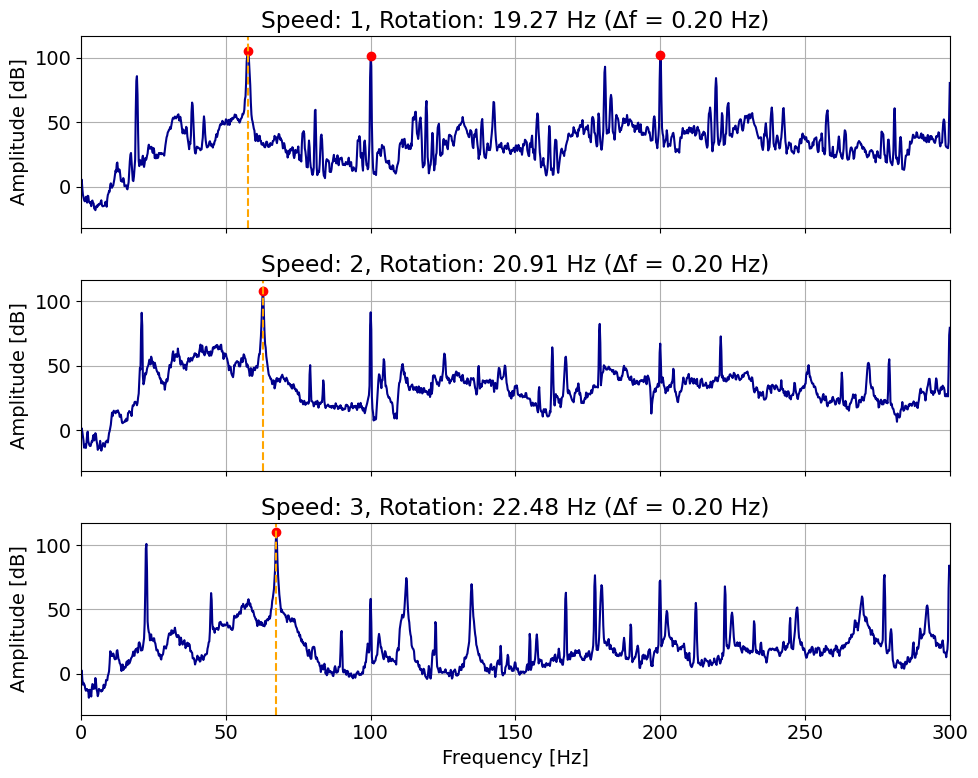
\includegraphics[width=\textwidth]{assets/results/standing-fan/standing-fan-accel.png}
        \caption{Estimation of rotation speed}
        \label{fig:evaluation:logger-fan-speed}
    \end{subfigure}
    \caption{Vibrations from the back of a standing fan in the radial direction}
\end{figure}

Time waveform captures mostly regular patterns of oscillatory motion  (Fig.~\ref{fig:evaluation:logger-waveform}). At slower speeds, the vibrations are higher because the fan is less stable and wobbles around the support. Timestamps from the sensor calibrate the sampling frequency from the theoretical 26667 Hz to the actual 26866 Hz. The estimate of fan rotational speed (Fig.~\ref{fig:evaluation:logger-fan-speed}) is accurate within the margin of error.

\subsection{Signal waveforms}
\begin{figure}[h]
    \centering
    \begin{subfigure}[b]{0.32\textwidth}
        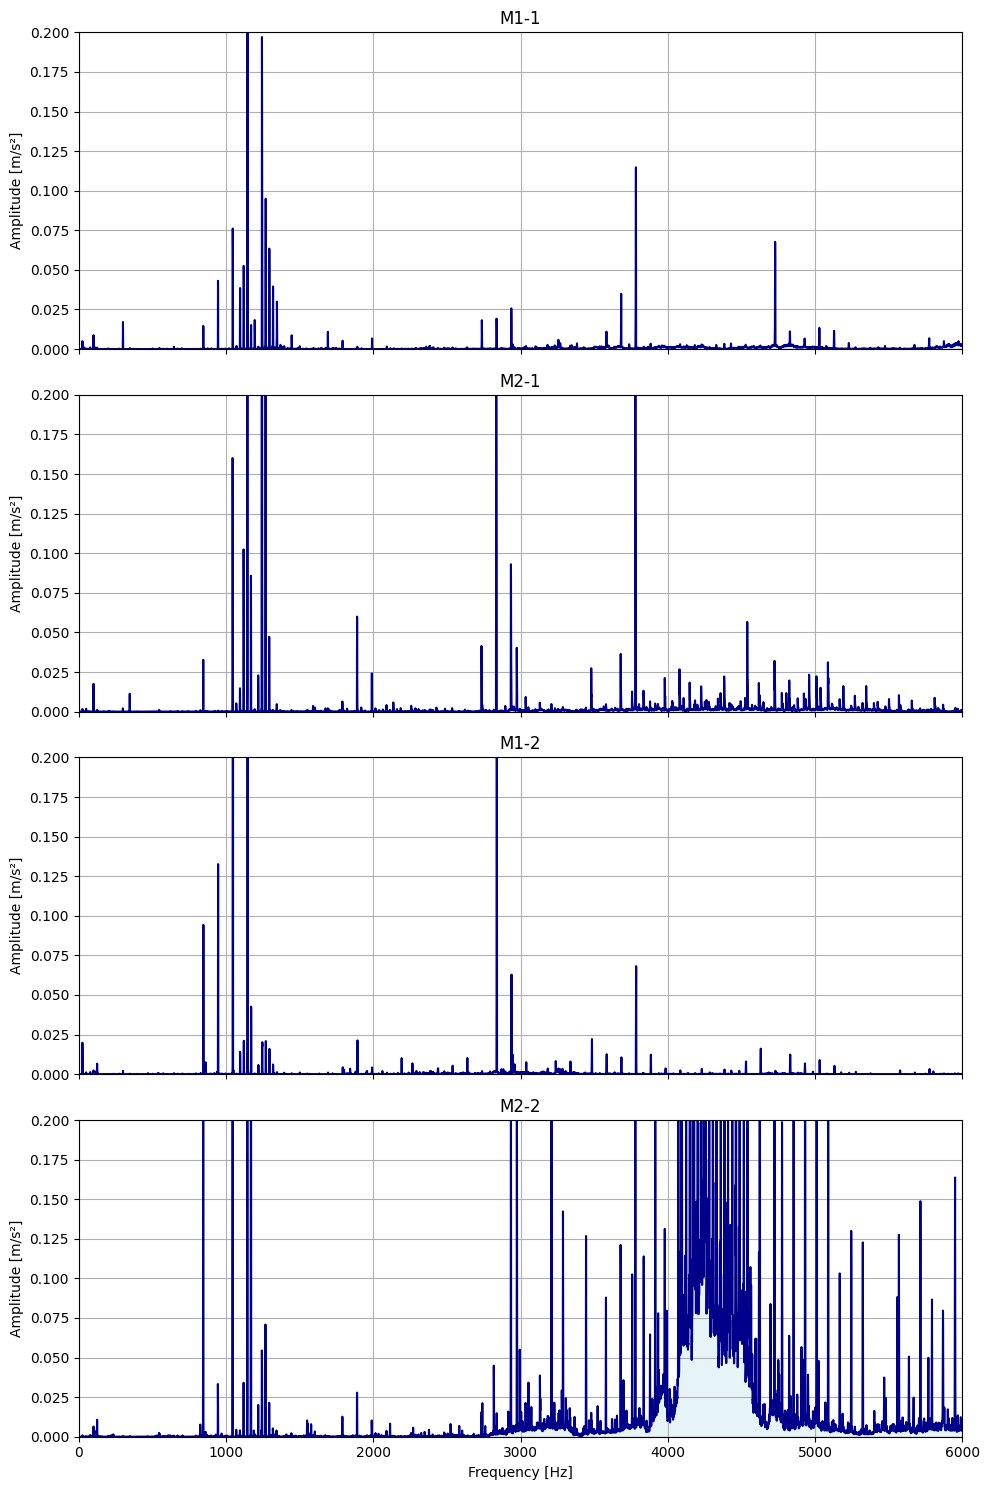
\includegraphics[width=\textwidth]{assets/results/eda/frequency-spectrum-motors.png}
        \caption{Motors}
    \end{subfigure}
    \hfill
    \begin{subfigure}[b]{0.32\textwidth}
        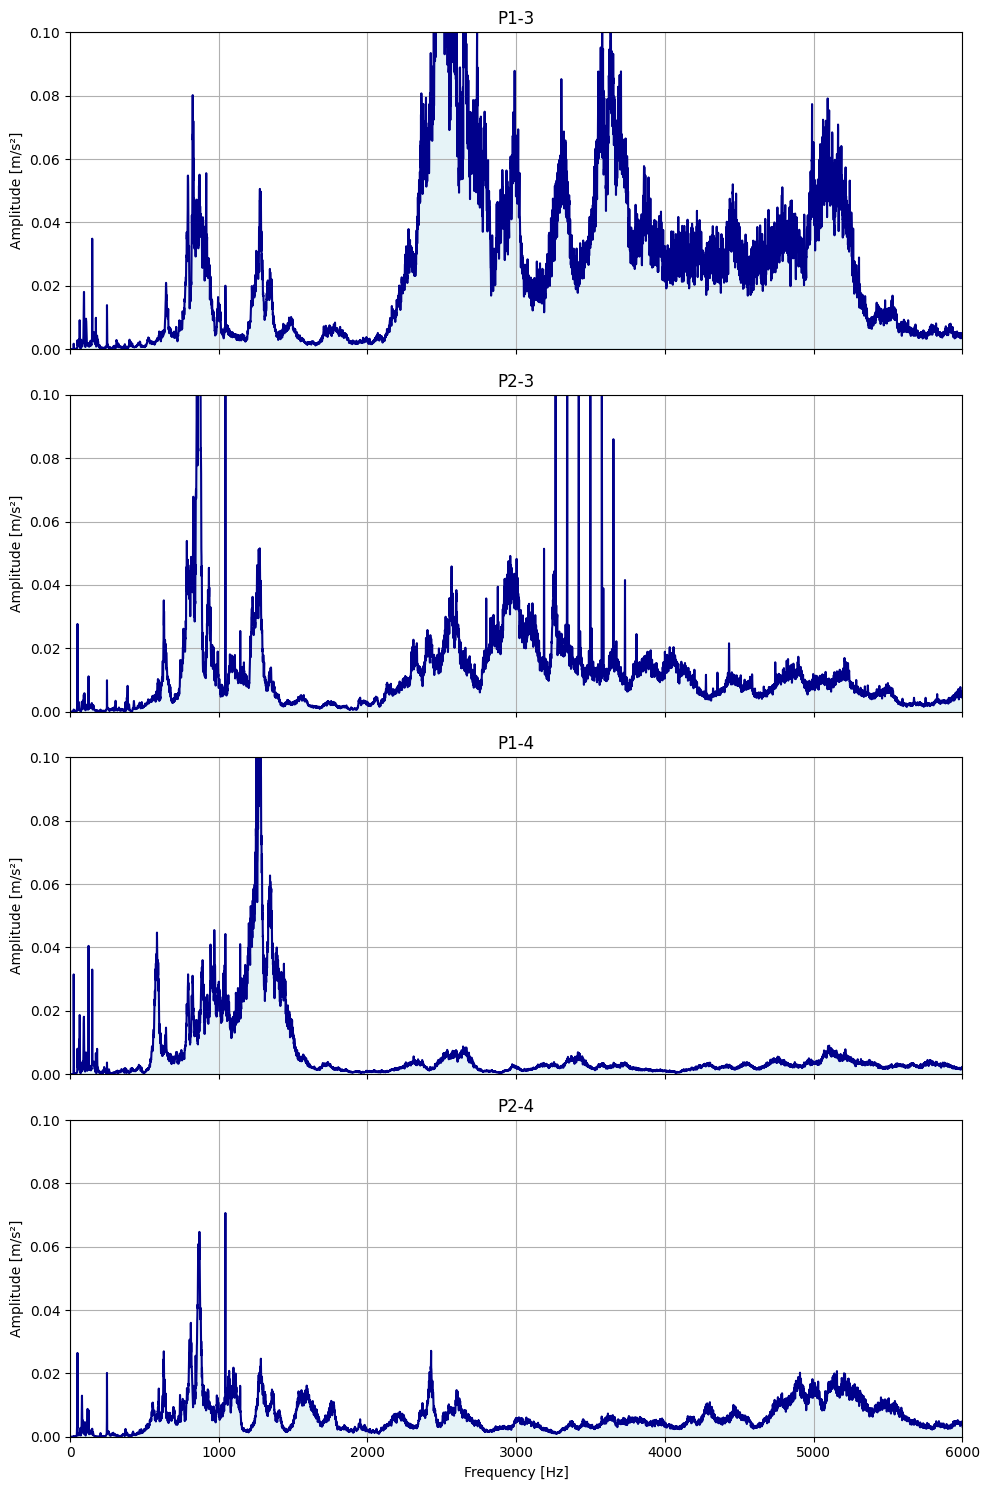
\includegraphics[width=\textwidth]{assets/results/eda/frequency-spectrum-pumps.png}
        \caption{Pumps}
    \end{subfigure}
    \hfill
    \begin{subfigure}[b]{0.32\textwidth}
        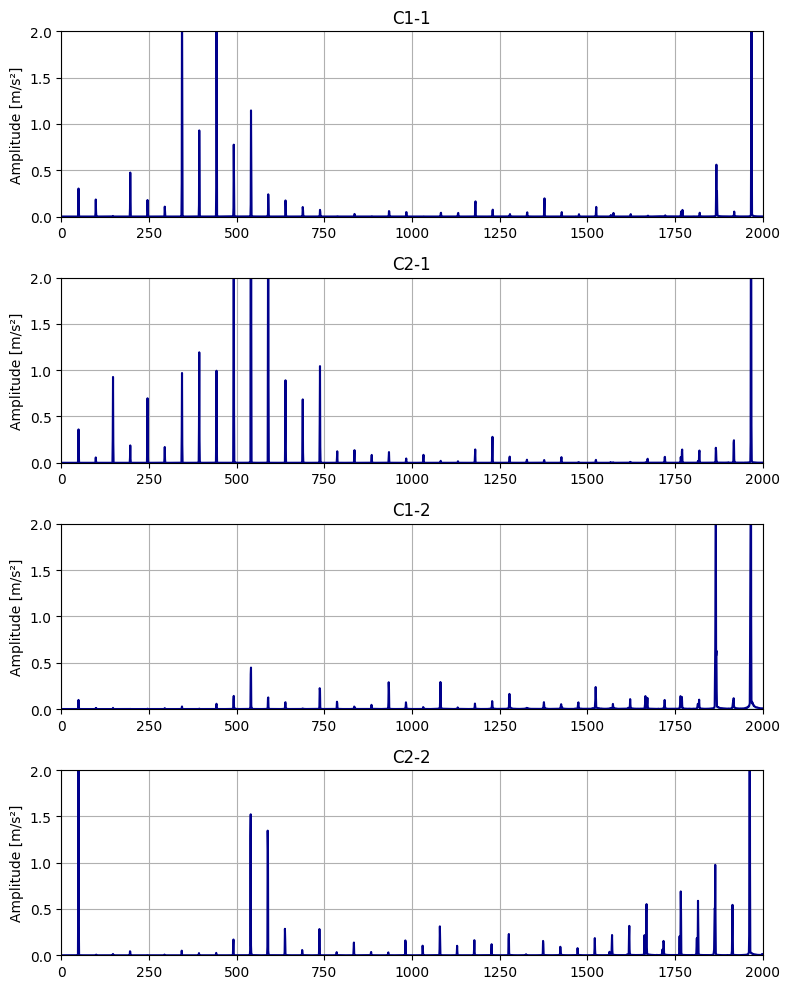
\includegraphics[width=\textwidth]{assets/results/eda/frequency-spectrum-compressors.png}
        \caption{Compressors}
    \end{subfigure} 
    \caption{Wideband frequency waveform of machinery vibartions in Pump dataset}
    \label{fig:evaluation:wideband-frequencies}
\end{figure}

The overview of wideband vibration frequency spectra from various sensor placements shows clear distinctions among the machines. The recordings in Figure~\ref{fig:evaluation:wideband-frequencies} present consistent shapes of waveforms found during repeated trials. The spectra are Welch's average of 32768 long windows with 50\% overlap over minute of recording.

The electric motor signals are polluted by noise from the wind blowing out of a large cooling fan at the back of the motor. The M2 in place two compared to M1 has elevated amplitudes above 4 kHz. The pumps have richer signal content than motors split into several frequency bands, likely due to the flow of water. The outer bearing (4) has a more attenuated amplitude above 1.5 kHz than the inner bearing (3). The P2 exhibits less vibration in comparable bands in general. The compressor casing produces a series of harmonics of rotational frequency, which are stronger near the scroll and suction valve than near the base.

\begin{table}[h]
\centering
\begin{tabular}{|l|r|r|r|}
\hline
\textbf{Placement}     & \multicolumn{1}{l|}{\textbf{M1}} & \multicolumn{1}{l|}{\textbf{M2}} & \multicolumn{1}{l|}{\textbf{P3, P4}} \\ \hline
\textbf{Bearing}       & \multicolumn{1}{l|}{6319-C3}            & \multicolumn{1}{l|}{6324-C3}            & \multicolumn{1}{l|}{6317-2Z}                  \\ \hline
\textbf{Rolling elements $n$}           & 8                                       & 8                                       & 8                                             \\ \hline
\textbf{Rotational speed $f_s$ {[}rpm{]}}         & 1493                                    & 1493                                    & 1493                                          \\ \hline
\textbf{Inner diameter $d$ {[}mm{]}}  & 33.12                                   & 41.28                                   & 30.00                                         \\ \hline
\textbf{Outer diameter$D$ {[}mm{]}}  & 147.5                                   & 190.0                                   & 132.5                                         \\ \hline
\textbf{Contact angle $\beta$}       & 0                                       & 0                                       & 0                                             \\ \hline
\textbf{RPM {[}Hz{]}}  & 24.88                                   & 24.88                                   & 24.88                                         \\ \hline
\textbf{BPFO {[}Hz{]}} & 77.18                                   & 77.91                                   & 77.00                                         \\ \hline
\textbf{BPFI {[}Hz{]}} & 121.88                                  & 121.16                                  & 122.07                                        \\ \hline
\textbf{BSF {[}Hz{]}}  & 58.20                                   & 59.97                                   & 57.77                                         \\ \hline
\textbf{FTF {[}Hz{]}}  & 9.65                                    & 9.74                                    & 9.63                                          \\ \hline
\end{tabular}
\caption{Bearing characteristic harmonic frequencies of pumps and their motors}
\label{tab:evaluation:bearing-freq-pump}
\end{table}

\begin{figure}[h]
    \centering
    \begin{subfigure}[b]{0.24\textwidth}
        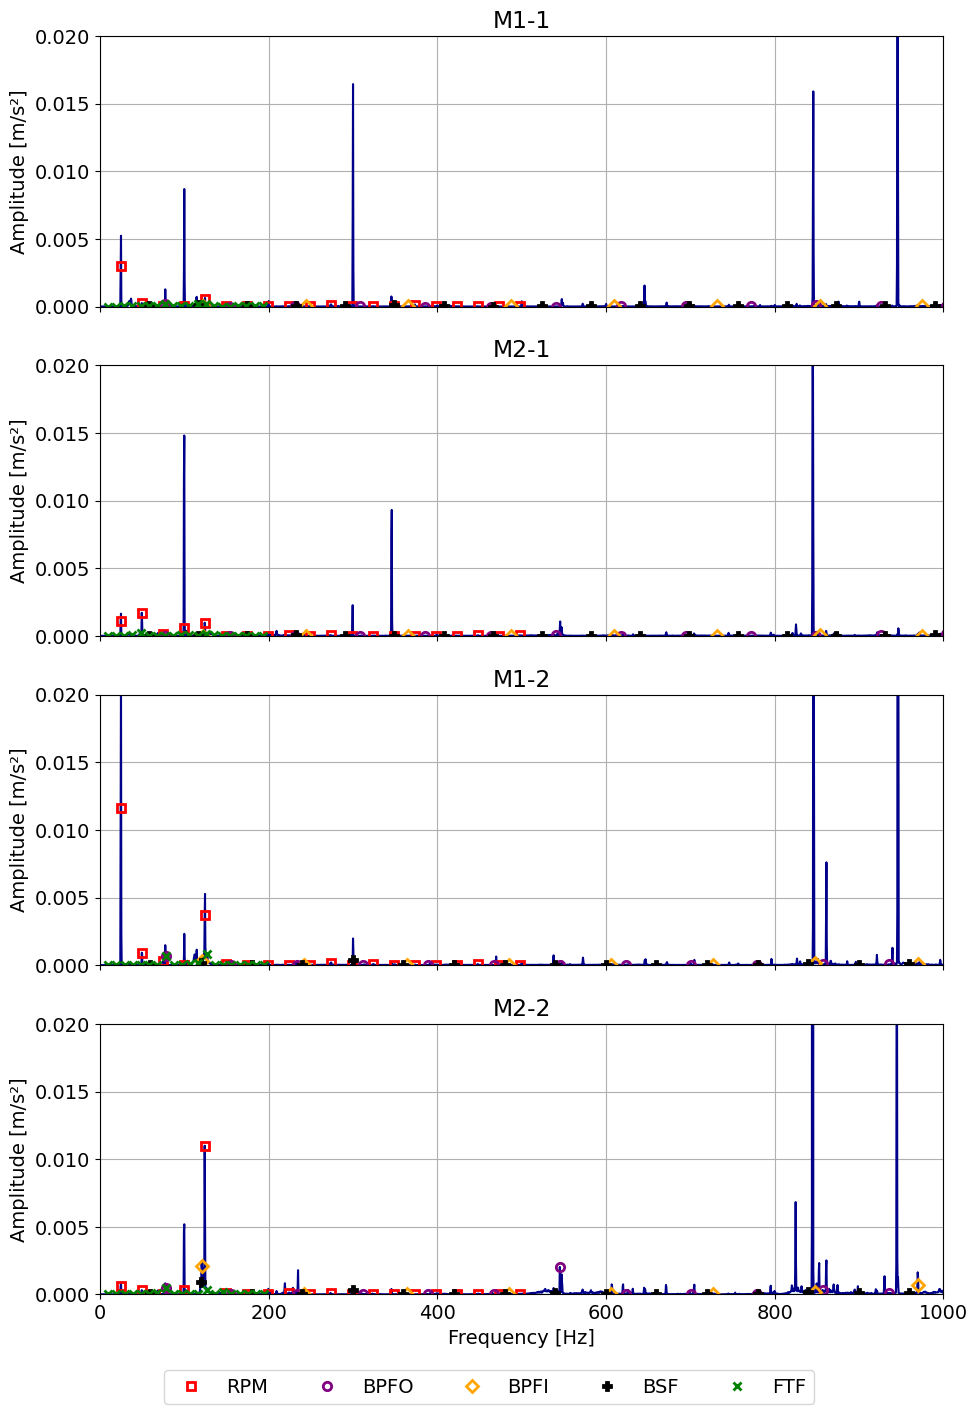
\includegraphics[width=\textwidth]{assets/results/defects/motors.png}
        \caption{Motors}
    \end{subfigure}
    \hfill
    \begin{subfigure}[b]{0.24\textwidth}
        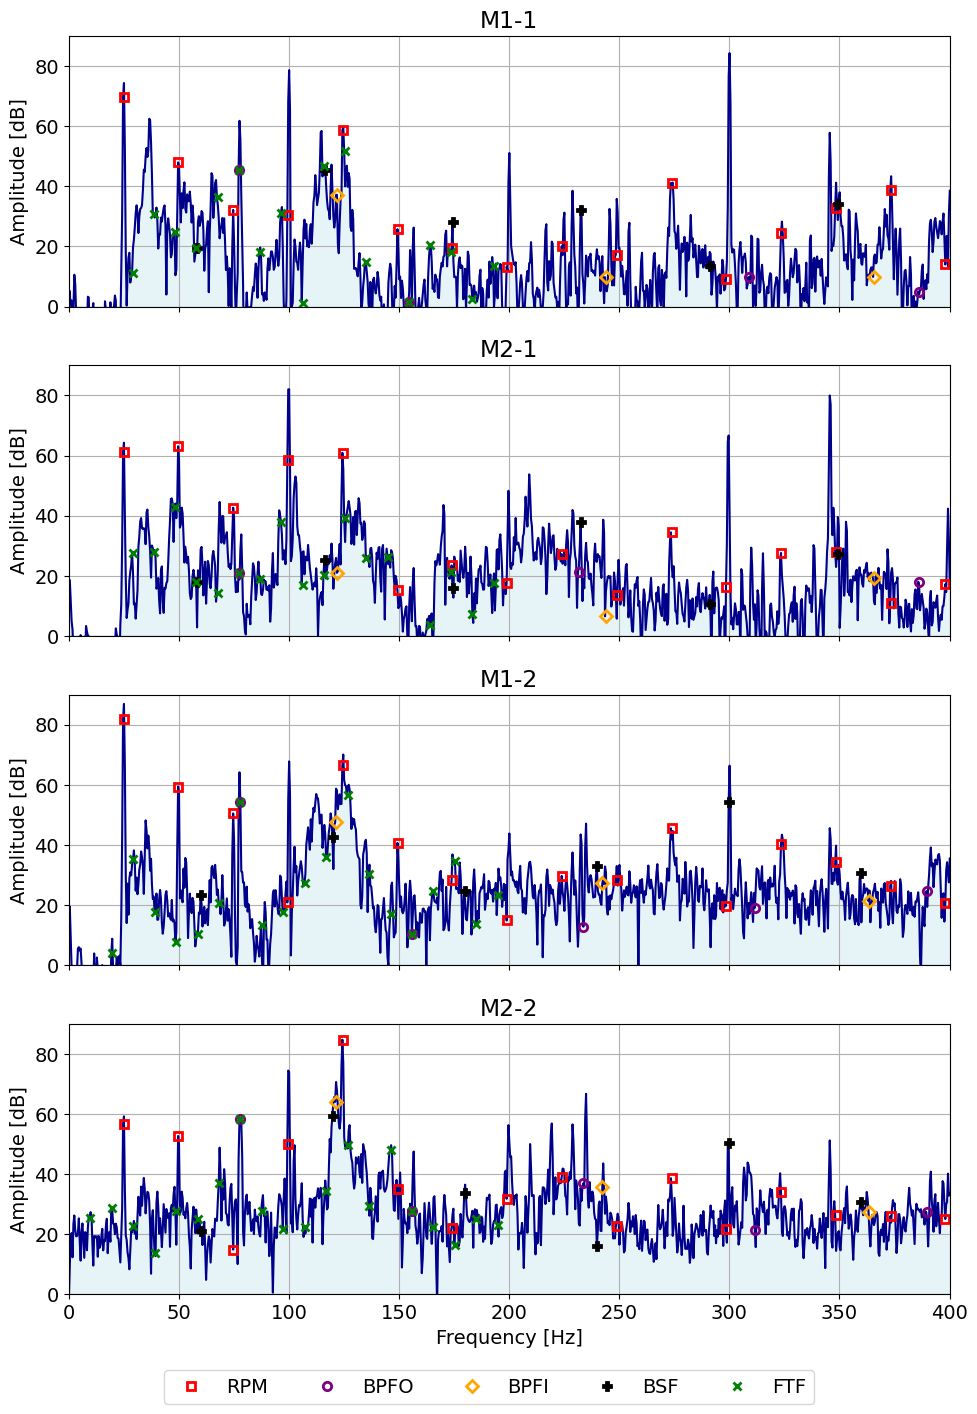
\includegraphics[width=\textwidth]{assets/results/defects/motors-dB.png}
        \caption{Motors (dB)}
    \end{subfigure}
    \begin{subfigure}[b]{0.24\textwidth}
        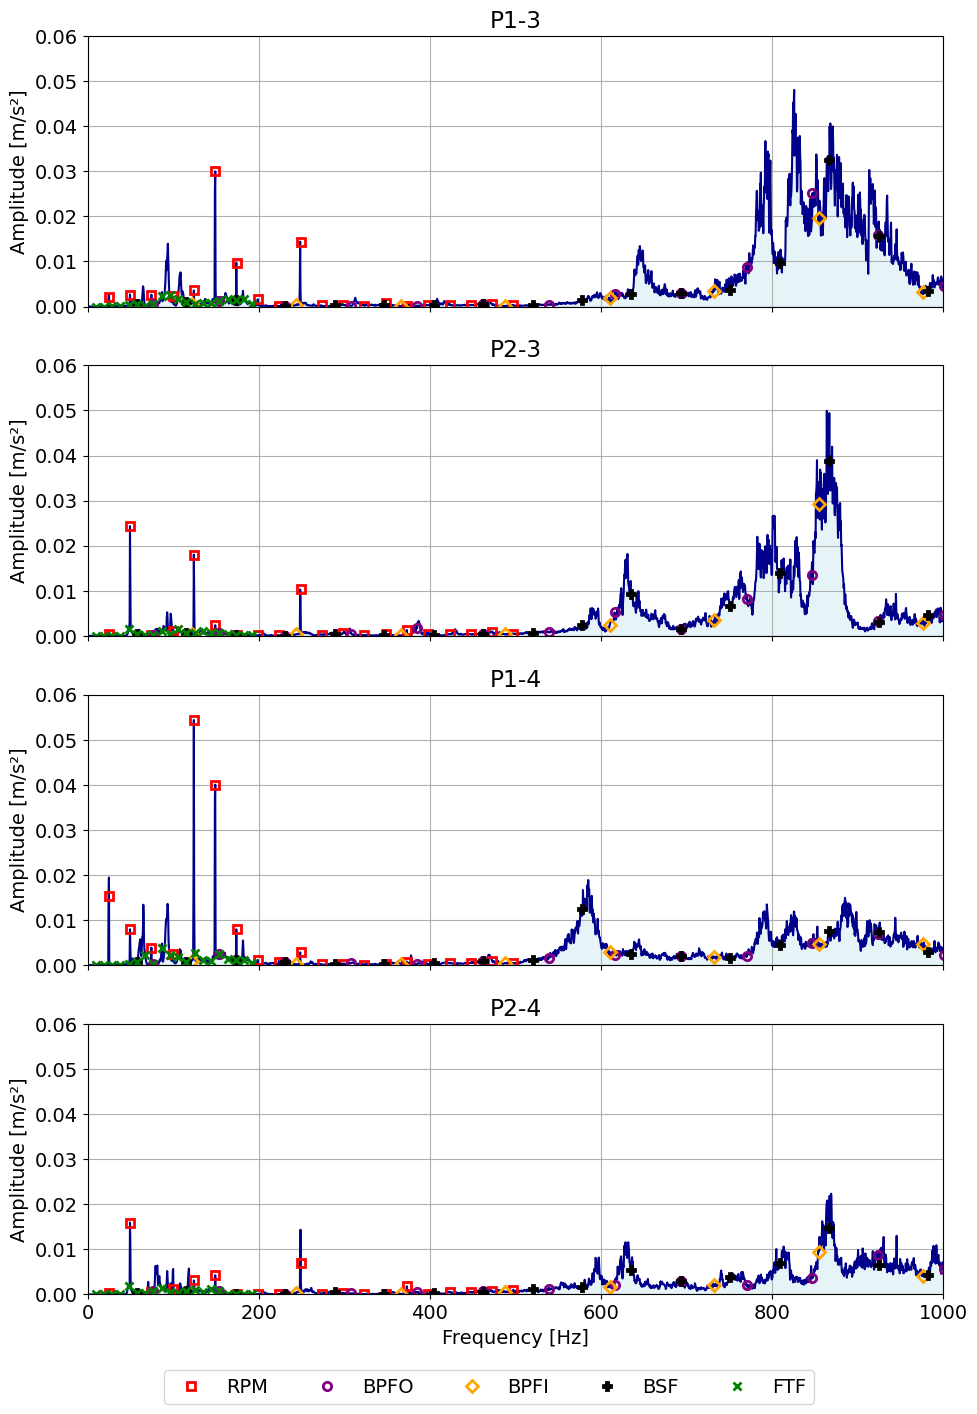
\includegraphics[width=\textwidth]{assets/results/defects/pumps.png}
        \caption{Pumps}
    \end{subfigure}
    \hfill
    \begin{subfigure}[b]{0.24\textwidth}
        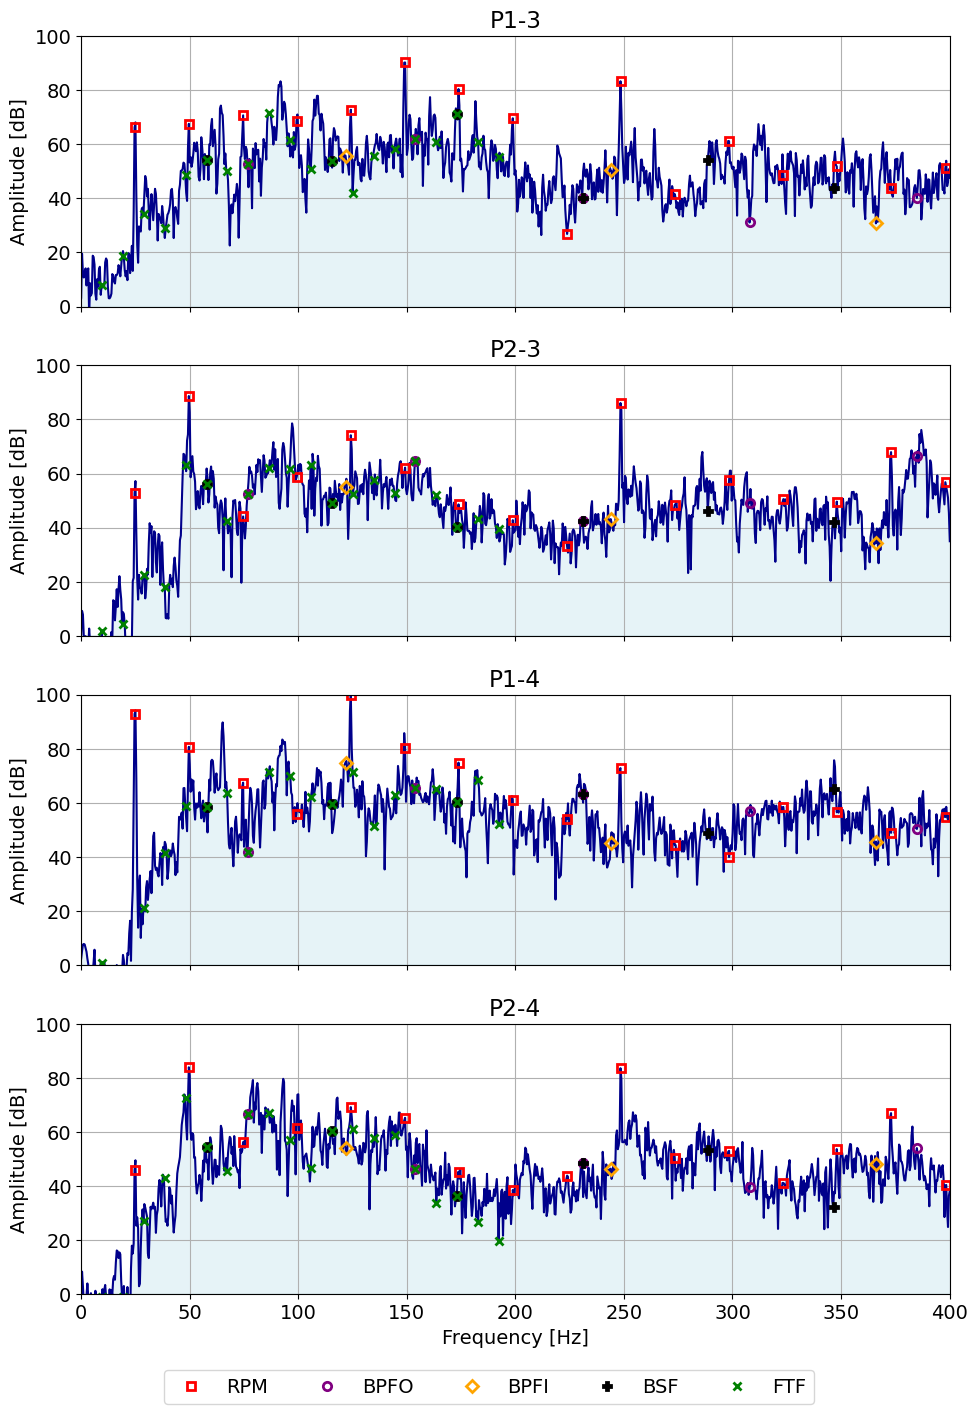
\includegraphics[width=\textwidth]{assets/results/defects/pumps-dB.png}
        \caption{Pumps (dB)}
    \end{subfigure}
    \caption{Characteric bearing frequencies of pumps}
    \label{fig:evaluation:bearing-freq}
\end{figure}

Domain experts recommended the procedure for fault identification by calculation of bearing characteristic frequencies (Tab.~\ref{tab:evaluation:bearing-freq-pump}), and they approved the following results. Figure~\ref{fig:evaluation:bearing-freq} identifies harmonics of rotational speed and BPFO frequency in every machine and BPFI for M2-2. It can be assumed that those frequencies will be the reason for damage in the future. The absolute acceleration is minuscule in current frequency bands and year-long sensor logs of rms velocity (Fig~\ref{fig:evaluation:ksb-guard-rms-vibartions}).

\begin{figure}[h]
    \centering
    \begin{subfigure}[b]{0.49\textwidth}
        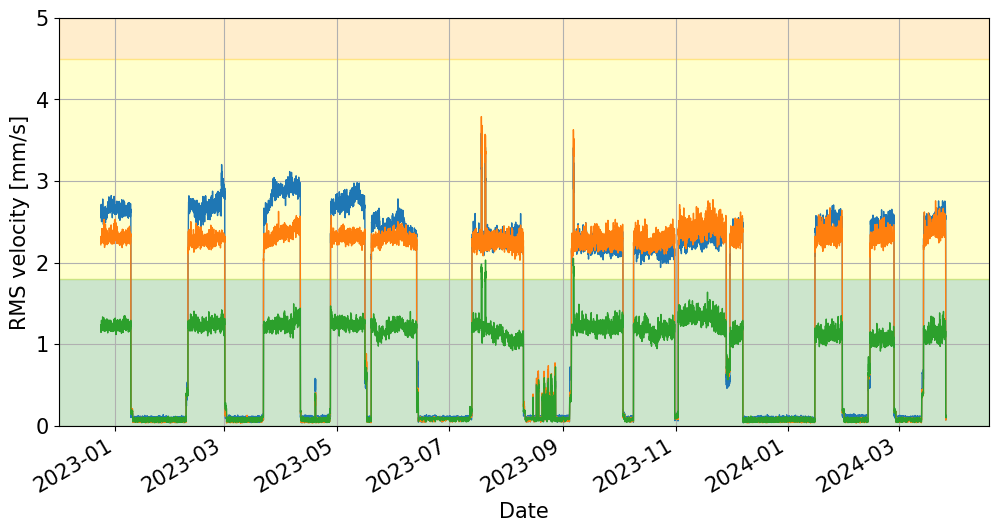
\includegraphics[width=\textwidth]{assets/results/ksb-cloud/p1.png}
        \caption{Pump P1}
    \end{subfigure}
    \hfill
    \begin{subfigure}[b]{0.49\textwidth}
        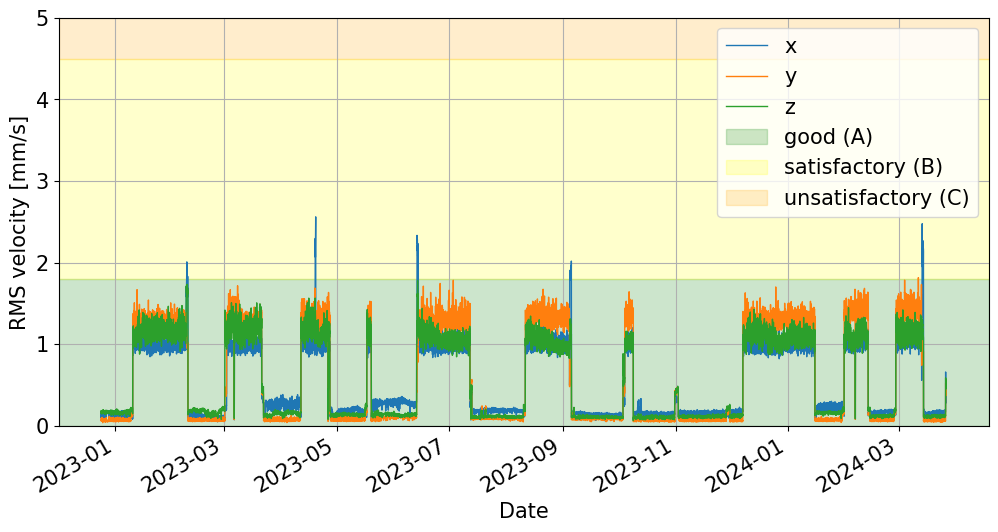
\includegraphics[width=\textwidth]{assets/results/ksb-cloud/p2.png}
        \caption{Pump P2}
    \end{subfigure}
    \caption{Vibration rms levels for a period over a year from KSB Guard}
    \label{fig:evaluation:ksb-guard-rms-vibartions}
\end{figure} 

Therefore, the current results suggest that the bearings are in flawless condition. During the over five years the pumps have been in service, there is not one instance of bearing fault due to rated lifespan and yearly prophylactic maintenance. This underscores the scarcity of recording faulty states in industrial environments. The monitoring is better suited in situations without preventive maintenance or with smaller machinery like the plunger pump BC~21/20S we considered during air conditioning inspections.

\begin{figure}[h]
    \centering
    \begin{subfigure}[b]{0.48\textwidth}
        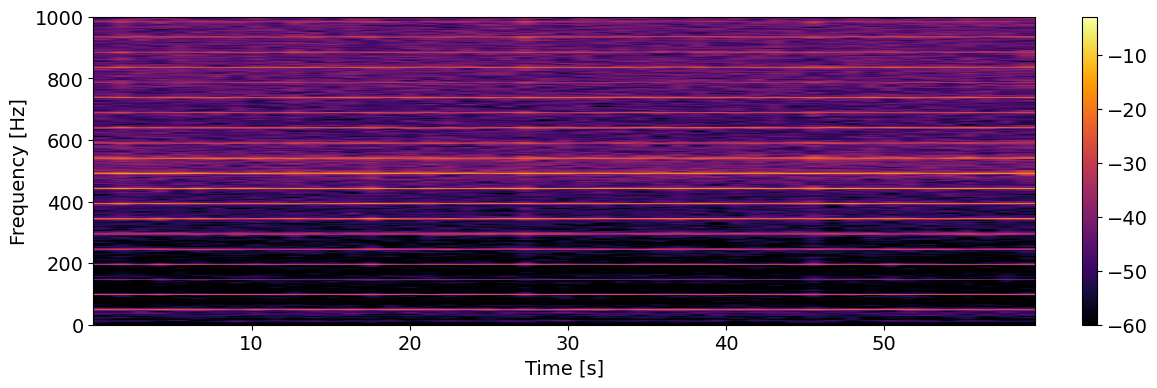
\includegraphics[width=\textwidth]{assets/results/time-frequency-spectrum/K3-z-STFT-1kHz.png}
        \caption{C1}
    \end{subfigure}
    \hfill
    \begin{subfigure}[b]{0.48\textwidth}
        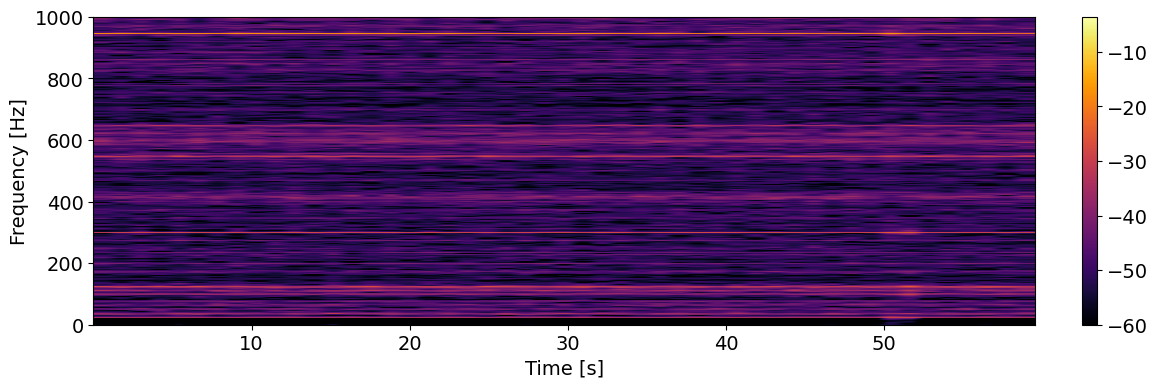
\includegraphics[width=\textwidth]{assets/results/time-frequency-spectrum/M1-2-z-STFT-1kHz.png}
        \caption{M1-2}
    \end{subfigure}
    \hfill
    \begin{subfigure}[b]{0.48\textwidth}
        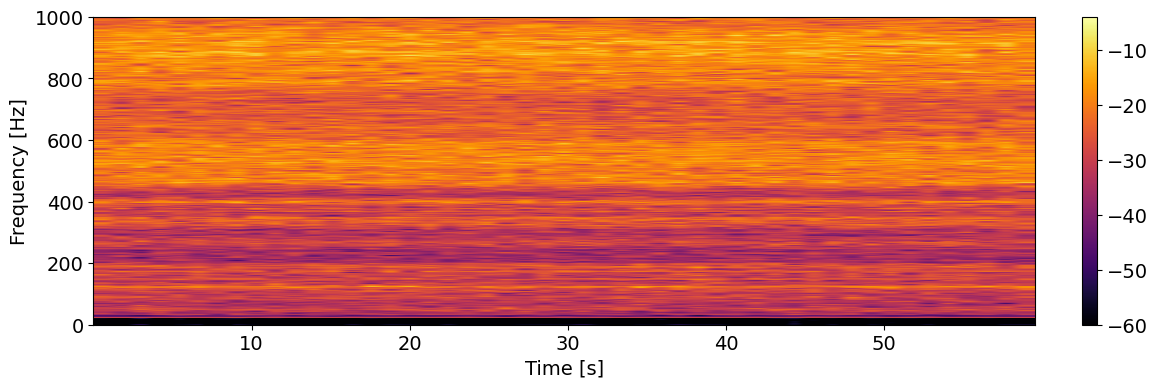
\includegraphics[width=\textwidth]{assets/results/time-frequency-spectrum/P1-3-z-STFT-1kHz.png}
        \caption{P1-3}
    \end{subfigure}
	\hfill
	\begin{subfigure}[b]{0.48\textwidth}
        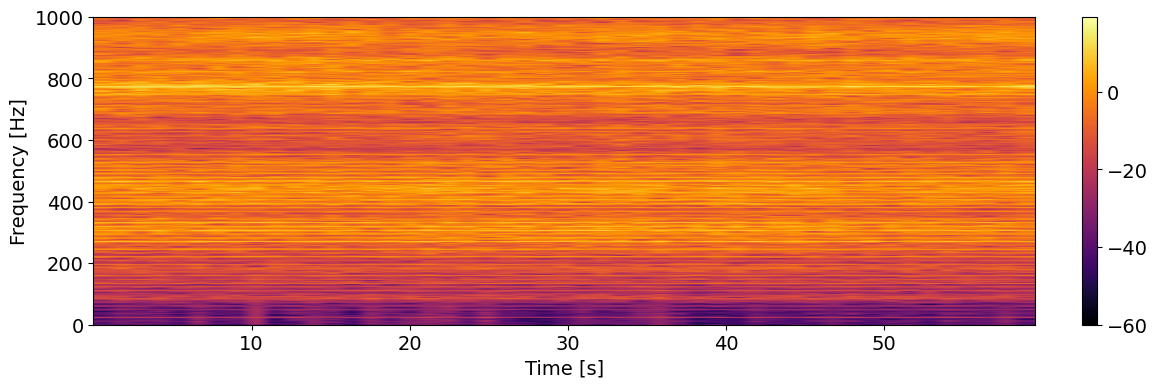
\includegraphics[width=\textwidth]{assets/results/time-frequency-spectrum/P3-3-z-STFT-1kHz.png}
        \caption{P3-3}
    \end{subfigure}
    \caption{Machinery vibration spectrograms ($f_s$ = 26.8~kHz, $w$ = 8~kS)}
    \label{fig:evaluation:spectrograms}
\end{figure}

Spectrograms point out that under constant machine load, the significant frequencies stay more or less unchanged over time (Fig~\ref{fig:evaluation:spectrograms}). The resolution of the uncertainty box is 306.95 ms and 3.26 Hz. Its magnitude is colored for decibel value.

\begin{figure}[h]
    \centering
    \begin{subfigure}[b]{0.48\textwidth}
        \includegraphics[width=\textwidth]{assets/results/time-frequency-spectrum/P1-slow-down.png}
        \caption{P1 turns off ($w$ = 4~kS)}
    \end{subfigure}
    \hfill
    \begin{subfigure}[b]{0.48\textwidth}
        \includegraphics[width=\textwidth]{assets/results/time-frequency-spectrum/P2-speed-up.png}
        \caption{P2 turns on ($w$ = 32~kS)}
        \label{fig:evaluation-sigma-pump-interference}
    \end{subfigure}
    \caption{Vibrations of water pumps during switch over ($f_s$ = 26.8~kHz)}
    \label{fig:evaluation:pump-switch-over}
\end{figure}

The water pump switch on and off creates a fast change in shaft speed. Resonance bands cannot be separated with enough time resolution by an automatic system at a chosen sampling rate. Due to inertia, slowing down takes about 10 seconds, whereas the speed up takes just half a second (Fig.~\ref{fig:evaluation:pump-switch-over}. The interference from excessive vibrations of the adjacent Sigma pump is picked up by the accelerometer on the KSB pump just before their switchover occurs (Fig~\ref{fig:evaluation-sigma-pump-interference}).

\begin{figure}[h]
    \centering
    \begin{subfigure}[b]{\textwidth}
        \includegraphics[width=\textwidth]{assets/results/feature-values/pumps-TD-dim-3.png}
        \caption{Time-domain features}
    \end{subfigure}
    \hfill
    \begin{subfigure}[b]{\textwidth}
        \includegraphics[width=\textwidth]{assets/results/feature-values/pumps-FD-dim-3.png}
        \caption{Frequency-domain features}
    \end{subfigure}
    \caption{The attribute value ranges of Pump dataset}
\end{figure}

The range of feature values for compressors and pumps are higher than in MaFaulDa despite most of them describing baseline status (Fig~\ref{fig:evaluation-sigma-pump-interference}). The increase can be seen for example in the interquartile range of rms (7.33 - 14.62 $\mathrm{m/s}^2$), centroid (3806 - 6003 Hz) or entropy (9.40 - 13.22 nats).